% SPDX-License-Identifier: GPL-3.0-or-later
\chapter{Nebuloase, Găuri Negre și Galaxii}
\label{chap:galaxii}

În \textbf{Orizontul 3 („Calea Lactee și Galaxii”)}, camera din \textbf{Orbitar} se ridică la mii și milioane de ani-lumină pentru a cuprinde arhitectura la scară mare a Universului: \textbf{nebuloasele difuze} (maternitățile cosmice unde se nasc mii de stele noi), \textbf{nebuloasele planetare și rămășițele de supernovă} (care îmbogățesc galaxia cu elementele chimice ale vieții), \textbf{gaura neagră supermasivă Sagittarius A*} din inima galaxiei noastre, \textbf{Calea Lactee} și \textbf{galaxiile vecine sau îndepărtate}.

\section*{De la Maternitățile de Stele la Galaxiile Spirale}

\begin{itemize}[leftmargin=1.5em, itemsep=3pt]
  \item \textbf{Nebuloasele de emisie și formare stelară (\emph{Orion M42, Stâlpii Creației M16, Carina NGC 3372}):} nori colosali de hidrogen rece și praf cosmic în care gravitația strânge materia în noduri dense numite protostele.
  \item \textbf{Nebuloasele planetare (\emph{Inelul M57, Helix NGC 7293}):} straturile exterioare luminoase de gaz eliberate pașnic la finalul vieții de stelele de mărimea Soarelui, lăsând în centru o \emph{pitică albă}.
  \item \textbf{Rămășițele de supernovă și pulsarii (\emph{Nebuloasa Crabului M1}):} explozii cataclismice ale stelelor masive, în urma cărora nucleul colapsează într-o \emph{stea neutronică (pulsar)} sau într-o \emph{gaură neagră}.
  \item \textbf{Roiurile globulare (precum \emph{Omega Centauri}):} sfere străvechi de până la $10\text{ milioane de stele}$ care orbitează în haloul Căii Lactee.
  \item \textbf{Galaxiile (\emph{Calea Lactee, Marele Nor al lui Magellan, Andromeda M31, Triunghiul M33, Vâltoarea M51, Sombrero M104}):} insule cosmice legate gravitațional, formate din zeci sau sute de miliarde de stele, gaz, praf, o gaură neagră supermasivă centrală și un halou invizibil de materie întunecată.
\end{itemize}

\begin{center}
\begin{tikzpicture}[scale=0.90, every node/.style={transform shape}]
  \fill[orbitarSpaceBg, rounded corners=6pt] (-1.0,-2.3) rectangle (13.6,2.3);

  % Discul Căii Lactee văzut de sus (schematic)
  \coordinate (G) at (3.6,0);
  \draw[white!20, line width=6pt] (G) circle (1.7cm);
  \draw[orbitarCyan!40, line width=3pt, dashed] (G) circle (1.25cm);
  \draw[orbitarAmber!60, line width=2pt] ($(G)+(-0.6,-0.25)$) -- ($(G)+(0.6,0.25)$);
  \fill[yellow!90!orange] (G) circle (0.28cm);
  \fill[black] (G) circle (0.09cm);
  \node[amber!90!yellow, font=\scriptsize\bfseries] at (3.6,-2.0) {Calea Lactee ($\sim$100.000 a.l. diametru)};

  % Poziția Soarelui în Brațul Orion
  \fill[orbitarCyan] ($(G)+(0.95,-0.55)$) circle (0.11cm);
  \draw[orbitarCyan, line width=0.8pt] ($(G)+(0.95,-0.55)$) circle (0.22cm);
  \draw[-{Stealth}, orbitarCyan, line width=0.8pt] (7.2,-0.8) -- ($(G)+(1.22,-0.58)$);
  \node[orbitarCyan, font=\scriptsize\bfseries, anchor=west, align=left] at (7.3,-0.8) {Sistemul nostru Solar (Acasă)\\în Brațul Orion (26.000 a.l. de centru)};

  % Săgeată spre Sagittarius A*
  \draw[-{Stealth}, amber!90!yellow, line width=0.8pt] (7.2,0.9) -- ($(G)+(0.25,0.15)$);
  \node[amber!90!yellow, font=\scriptsize\bfseries, anchor=west, align=left] at (7.3,0.9) {Gaura Neagră Sagittarius A*\\(4,3 milioane mase solare)};
\end{tikzpicture}
\end{center}

\begin{table}[H]
\centering
\small
\caption{Cele 13 nebuloase, găuri negre și galaxii din Orizontul 3 în Orbitar}
\resizebox{\textwidth}{!}{%
\begin{tabular}{@{}lll@{}}
\toprule
\textbf{Obiect Cosmic} & \textbf{Categorie} & \textbf{Distanță / Scară în Ani-Lumină} \\
\midrule
Nebuloasa Orion (M42) & Nebuloasă Cosmică & 1.344 de ani-lumină \\
Stâlpii Creației (Nebuloasa Vulturului M16) & Nebuloasă Cosmică & 6.500 de ani-lumină \\
Sagittarius A* (Gaura Neagră Supermasivă) & Gaură Neagră Supermasivă & 26.000 de ani-lumină \\
Calea Lactee (Galaxia Noastră) & Galaxie & Diametru aproximativ 100.000 ani-lumină (Soarele la 26.000 a.l. de centru) \\
Galaxia Andromeda (M31) & Galaxie & 2,54 de milioane de ani-lumină \\
Nebuloasa Carina (\quotedblbase{}Stâncile Cosmice\textquotedblright{}, NGC 3372) & Nebuloasă Cosmică & 7.500 de ani-lumină \\
Nebuloasa Crabului (M1) & Nebuloasă Cosmică & 6.500 de ani-lumină \\
Nebuloasa Inelul (M57) & Nebuloasă Cosmică & 2.300 de ani-lumină \\
Nebuloasa Helix (\quotedblbase{}Ochiul lui Dumnezeu\textquotedblright{}, NGC 7293) & Nebuloasă Cosmică & 650 de ani-lumină \\
Marele Nor al lui Magellan & Galaxie & 160.000 de ani-lumină \\
Galaxia Triunghiului (M33) & Galaxie & 2,73 de milioane de ani-lumină \\
Galaxia Vâltoarea (M51) & Galaxie & 23,5 milioane de ani-lumină \\
Galaxia Sombrero (M104) & Galaxie & 29,3 milioane de ani-lumină \\
\bottomrule
\end{tabular}%
}
\end{table}

\clearpage

\section{Nebuloasa Orion (M42)}
\label{sec:body-orion_nebula}
\vspace{-4pt}
{\large\itshape\color{orbitarAccent} Cea mai apropiată maternitate stelară masivă, studiată de James Webb (1.344 ani-lumină)}\\[4pt]


\begin{center}
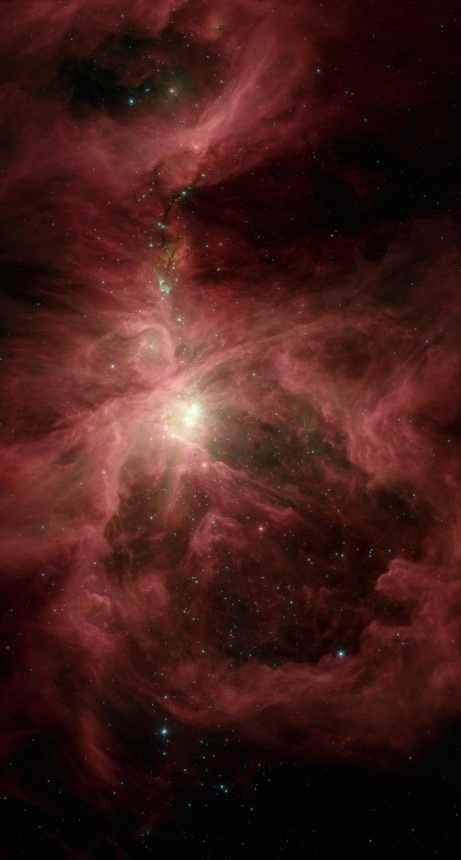
\includegraphics[width=0.78\textwidth,height=5.6cm,keepaspectratio]{../public/textures/nasa/orion_nebula.jpg}\\[3pt]
{\footnotesize\itshape\color{orbitarMuted} Fotografie reală NASA/JPL-Caltech/ESA (Hubble \& Spitzer PIA08653): Maternitatea stelară Nebuloasa Orion (M42).}
\end{center}


\begin{tcolorbox}[orbitardata, title={\textbf{Repere esențiale: Nebuloasa Orion (M42)}}]
\small
\begin{itemize}[leftmargin=1.4em, itemsep=2pt, topsep=2pt]
  \item \textbf{Clasificare și orbită:} Nebuloasă Cosmică \quad$\bullet$\quad \textbf{Distanță:} 1.344 de ani-lumină
  \item \textbf{Dimensiuni și masă:} Nebuloasa Orion măsoară 24 de ani-lumină de la un capăt la altul și este de 24 de ori mai lată decât întregul Sistem Solar împreună cu Norul lui Oort! \quad$\bullet$\quad masă: 666000000,000 $\times M_\oplus$
  \item \textbf{Gravitație și regim termic:} 0,100 $\times g_\oplus$ (0,98 m/s$^2$) \quad$\bullet$\quad temperatură medie: +9.700 $^\circ$C
  \item \textbf{Ciclu orbital și rotație:} perioadă orbitală (an): Orbitează centrul Căii Lactee (aproximativ 230 de milioane de ani) \quad$\bullet$\quad rotație (zi): 24,00 ore (1,00 zile pământești)
  \item \textbf{Durata călătoriei de pe Pământ:} cu viteza luminii ($1c$): \emph{1.344 de ani}; cu racheta ($50.000$ de kilometri pe oră): \emph{24 de milioane de ani}; cu avionul ($900$ de kilometri pe oră): \emph{1.680 de miliarde de ani}; cu mașina ($100$ de kilometri pe oră): \emph{15.000 de miliarde de ani}.
  \item \textbf{Repere de scară și curiozitate:} Nebuloasa Orion este ca un cuib luminos din vată de zahăr cosmică, lat de 24 de ani-lumină, în mijlocul căruia patru stele-bebeluș foarte puternice (\quotedblbase{}Trapezul\textquotedblright{}) aprind întregul nor ca niște reflectoare! Telescopul Spațial James Webb a privit cu ochii săi în infraroșu în interiorul Nebuloasei Orion și a fotografiat discuri de praf (\quotedblbase{}proplyde\textquotedblright{}) în jurul stelelor nou-născute, exact acolo unde se formează viitoare planete!
\end{itemize}
\end{tcolorbox}

\vspace{4pt}
\noindent\textbf{Prezentare generală și profil astrofizic.} Nebuloasa Orion (Messier 42 / NGC 1976), situată la 1.344 de ani-lumină, este cea mai strălucitoare nebuloasă difuză de emisie și reflexie de pe cer (vizibilă chiar și cu ochiul liber, magnitudine 4,0). În centrul ei, roiul tânăr Trapezium ionizează hidrogenul și oxigenul din jur, iar observațiile JWST NIRCam au dezvăluit filamente moleculare, jeturi protostelare și discuri protoplanetare. Sub cele trei stele din \quotedblbase{}Centura lui Orion\textquotedblright{} se află un nor cosmic uriaș, strălucitor în nuanțe de roz, violet și turcoaz: Nebuloasa Orion! Este o adevărată \quotedblbase{}maternitate de stele\textquotedblright{}, un loc fermecat în care din nori de gaz și praf cosmic se nasc chiar acum sute de sori noi și sisteme solare tinere! Nebuloasa Orion este ca un cuib luminos din vată de zahăr cosmică, lat de 24 de ani-lumină, în mijlocul căruia patru stele-bebeluș foarte puternice (\quotedblbase{}Trapezul\textquotedblright{}) aprind întregul nor ca niște reflectoare!

\medskip
\noindent\textbf{Scara cosmică și călătoria luminii în timp.} La scară astronomică, dimensiunile sale sunt impresionante: Nebuloasa Orion măsoară 24 de ani-lumină de la un capăt la altul și este de 24 de ori mai lată decât întregul Sistem Solar împreună cu Norul lui Oort! Totodată, privind astăzi spre Nebuloasa Orion (M42), observăm practic trecutul îndepărtat al Universului, întrucât lumina sa a călătorit prin spațiu până la noi: Lumina de la Nebuloasa Orion pe care o vedem azi a plecat acum 1.344 de ani (în anul 682 d.Hr.), în secolele în care se forma poporul român și limba română!

\medskip
\noindent\textbf{Alcătuirea fizică și structura internă.} Privind în profunzimea sa, alcătuirea fizică este organizată pe mai multe straturi și regiuni distincte, fiecare având un rol bine definit în evoluția și dinamica acestui obiect cosmic. În primul rând se remarcă \textbf{Roiul Stelar Trapezium}, grup compact de stele masive tinere (tip O și B) a căror radiație ultravioletă face întreaga nebuloasă să strălucească. În completarea acestui ansamblu întâlnim \textbf{Bara Orion \& Discurile Protoplanetare (Proplyds)}, peste 150 de discuri de praf și gaz în jurul stelelor tinere, unde se nasc noi planete, fotografiate în detaliu de Hubble și James Webb.

\medskip
\noindent\textbf{Observații astronomice și istoricul explorării.} Observată prin telescop în 1610 de Nicolas-Claude Fabri de Peiresc și desenată de Christiaan Huygens în 1656; în 2022--2023, Telescopul Spațial James Webb a realizat cele mai detaliate hărți în infraroșu ale regiunii. Telescopul Spațial James Webb a privit cu ochii săi în infraroșu în interiorul Nebuloasei Orion și a fotografiat discuri de praf (\quotedblbase{}proplyde\textquotedblright{}) în jurul stelelor nou-născute, exact acolo unde se formează viitoare planete!

\vspace{6pt}
\begin{tcolorbox}[orbitarquiz, title={\textbf{Întrebare de verificare \#54: Nebuloasa Orion (M42)}}]
\textbf{Ce se întâmplă în interiorul Nebuloasei Orion (M42), studiată de Telescopul James Webb?}
\begin{itemize}[leftmargin=2.2em, itemsep=2pt, topsep=4pt]
  \item[$\square$ \textbf{A.}] Se nasc sute de stele noi și sisteme planetare tinere din nori de gaz și praf cosmic
  \item[$\square$ \textbf{B.}] Se află doar planete înghețate fără nicio stea
  \item[$\square$ \textbf{C.}] Este o stație spațială pe orbita Pământului
  \item[$\square$ \textbf{D.}] Este un crater de pe Luna noastră
\end{itemize}
\vspace{2pt}
{\footnotesize\color{orbitarMuted}\textbf{Răspuns corect:} \textbf{A} (Se nasc sute de stele noi și sisteme planetare tinere din nori de gaz și praf cosmic). \emph{Nebuloasa Orion este cea mai apropiată regiune masivă de formare a stelelor (\quotedblbase{}maternitate stelară\textquotedblright{}), unde JWST observă stele nou-născute și discuri protoplanetare.}}
\end{tcolorbox}
\clearpage


\section{Stâlpii Creației (Nebuloasa Vulturului M16)}
\label{sec:body-pillars_of_creation}
\vspace{-4pt}
{\large\itshape\color{orbitarAccent} Coloanele gigantice de gaz și praf în care se nasc stele noi (6.500 ani-lumină)}\\[4pt]


\begin{center}
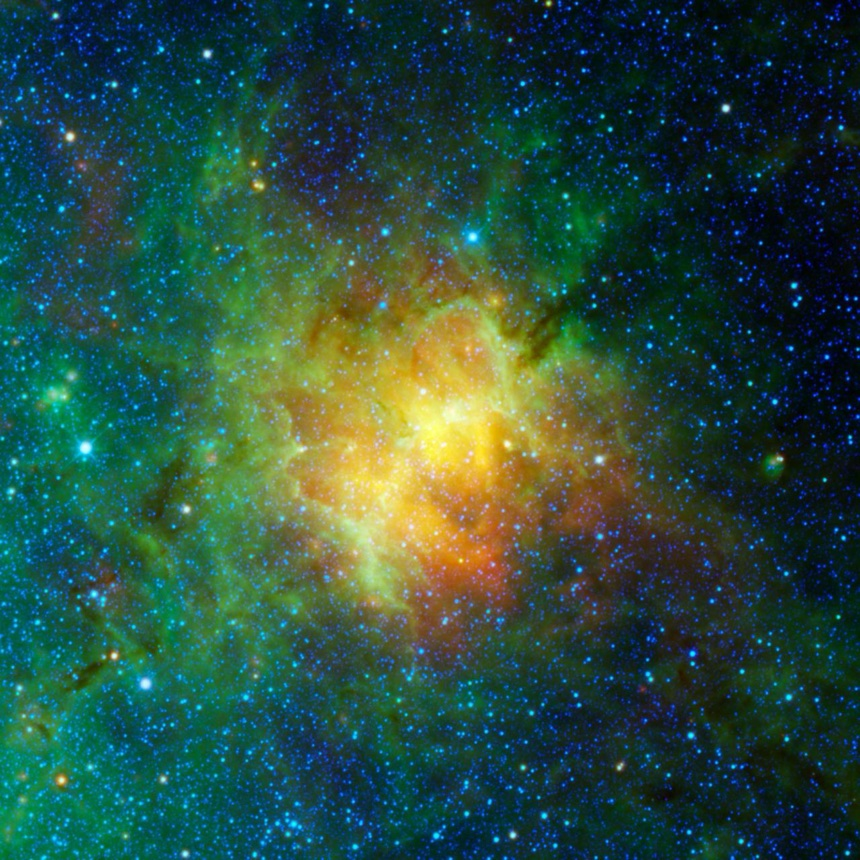
\includegraphics[width=0.78\textwidth,height=5.6cm,keepaspectratio]{../public/textures/nasa/pillars_of_creation.jpg}\\[3pt]
{\footnotesize\itshape\color{orbitarMuted} Fotografie reală NASA/ESA/CSA/STScI (Telescopul Spațial James Webb, PIA25433): \quotedblbase{}Stâlpii Creației\textquotedblright{} din Nebuloasa Vulturului (M16).}
\end{center}


\begin{tcolorbox}[orbitardata, title={\textbf{Repere esențiale: Stâlpii Creației (Nebuloasa Vulturului M16)}}]
\small
\begin{itemize}[leftmargin=1.4em, itemsep=2pt, topsep=2pt]
  \item \textbf{Clasificare și orbită:} Nebuloasă Cosmică \quad$\bullet$\quad \textbf{Distanță:} 6.500 de ani-lumină
  \item \textbf{Dimensiuni și masă:} Cel mai înalt stâlp are o lungime de aproximativ 4--5 ani-lumină, egală cu distanța de la Soarele nostru până la cea mai apropiată stea, Proxima Centauri! \quad$\bullet$\quad masă: 200000000,000 $\times M_\oplus$
  \item \textbf{Gravitație și regim termic:} 0,100 $\times g_\oplus$ (0,98 m/s$^2$) \quad$\bullet$\quad temperatură medie: +8.000 $^\circ$C
  \item \textbf{Ciclu orbital și rotație:} perioadă orbitală (an): Orbitează centrul Căii Lactee (aproximativ 230 de milioane de ani) \quad$\bullet$\quad rotație (zi): 24,00 ore (1,00 zile pământești)
  \item \textbf{Durata călătoriei de pe Pământ:} cu viteza luminii ($1c$): \emph{6.500 de ani}; cu racheta ($50.000$ de kilometri pe oră): \emph{117 milioane de ani}; cu avionul ($900$ de kilometri pe oră): \emph{8.100 de miliarde de ani}; cu mașina ($100$ de kilometri pe oră): \emph{73.000 de miliarde de ani}.
  \item \textbf{Repere de scară și curiozitate:} Stâlpii Creației seamănă cu trei munți de nori aurii ridicați în mijul cosmosului, atât de înalți încât o rază de lumină are nevoie de 5 ani întregi ca să urce de la baza unui stâlp până în vârful lui! Când Telescopul James Webb a privit Stâlpii Creației în lumină infraroșie, praful a devenit transparent și au apărut mii de stele tinere roșii ascunse chiar în interiorul coloanelor!
\end{itemize}
\end{tcolorbox}

\vspace{4pt}
\noindent\textbf{Prezentare generală și profil astrofizic.} Situați la aproximativ 6.500 de ani-lumină în Nebuloasa Vulturului (Messier 16, constelația Șarpele), Stâlpii Creației sunt trompe elefantine de hidrogen molecular rece și praf cosmic, sculptate prin fotoevaporare de vânturile stelare și radiația UV ale stelelor masive din roiul NGC 6611. Imaginile JWST (NIRCam și MIRI, 2022) au evidențiat protostele de clasă 0/I la extremitățile stâlpilor. Stâlpii Creației sunt trei turnuri uriașe de gaz și praf stelar din inima Nebuloasei Vulturului, devenite celebre în toată lumea datorită fotografiilor uimitoare realizate de telescoapele Hubble și James Webb! În vârful acestor coloane aurii și turcoaz, înalte de câțiva ani-lumină, se aprind stele noi-nouțe, roșii ca jarul! Stâlpii Creației seamănă cu trei munți de nori aurii ridicați în mijul cosmosului, atât de înalți încât o rază de lumină are nevoie de 5 ani întregi ca să urce de la baza unui stâlp până în vârful lui!

\medskip
\noindent\textbf{Scara cosmică și călătoria luminii în timp.} La scară astronomică, dimensiunile sale sunt impresionante: Cel mai înalt stâlp are o lungime de aproximativ 4--5 ani-lumină, egală cu distanța de la Soarele nostru până la cea mai apropiată stea, Proxima Centauri! Totodată, privind astăzi spre Stâlpii Creației (Nebuloasa Vulturului M16), observăm practic trecutul îndepărtat al Universului, întrucât lumina sa a călătorit prin spațiu până la noi: Lumina de la Stâlpii Creației pe care o vedem azi a plecat acum 6.500 de ani (în jurul anului 4500 î.Hr.), pe vremea străvechii culturi Cucuteni de pe teritoriul României!

\medskip
\noindent\textbf{Alcătuirea fizică și structura internă.} Privind în profunzimea sa, alcătuirea fizică este organizată pe mai multe straturi și regiuni distincte, fiecare având un rol bine definit în evoluția și dinamica acestui obiect cosmic. În primul rând se remarcă \textbf{Coloanele Moleculare (4--5 ani-lumină)}, trei piloni denși de hidrogen molecular și praf cosmic care protejează gazul din spate de radiația ultravioletă. În completarea acestui ansamblu întâlnim \textbf{Globule de Gaz în Evaporare (EGGs) \& Protostele}, noduri dense la vârful stâlpilor în care gravitația comprimă gazul, dând naștere unor stele tinere vizibile în infraroșu cu JWST.

\medskip
\noindent\textbf{Observații astronomice și istoricul explorării.} Fotografia iconică realizată de Telescopul Spațial Hubble în 1995 (și refăcută în 2014) a fost completată în octombrie 2022 de imaginea în infraroșu apropiat și mediu a Telescopului Spațial James Webb. Când Telescopul James Webb a privit Stâlpii Creației în lumină infraroșie, praful a devenit transparent și au apărut mii de stele tinere roșii ascunse chiar în interiorul coloanelor!

\vspace{6pt}
\begin{tcolorbox}[orbitarquiz, title={\textbf{Întrebare de verificare \#55: Stâlpii Creației (Nebuloasa Vulturului M16)}}]
\textbf{Ce a reușit să vadă Telescopul Spațial James Webb în interiorul Stâlpilor Creației folosind lumina infraroșie?}
\begin{itemize}[leftmargin=2.2em, itemsep=2pt, topsep=4pt]
  \item[$\square$ \textbf{A.}] A privit prin perdeaua de praf și a dezvăluit stelele tinere roșii care se nasc în vârful coloanelor
  \item[$\square$ \textbf{B.}] A descoperit un ocean de apă înghețată pe Marte
  \item[$\square$ \textbf{C.}] A fotografiat Stația Spațială Internațională
  \item[$\square$ \textbf{D.}] A măsurat coada unei comete din Centura Kuiper
\end{itemize}
\vspace{2pt}
{\footnotesize\color{orbitarMuted}\textbf{Răspuns corect:} \textbf{A} (A privit prin perdeaua de praf și a dezvăluit stelele tinere roșii care se nasc în vârful coloanelor). \emph{Lumina infraroșie pătrunde prin norii opaci de praf cosmic, permițând telescopului James Webb să fotografieze protostelele roșii nou-născute din interiorul Stâlpilor Creației.}}
\end{tcolorbox}
\clearpage


\section{Sagittarius A* (Gaura Neagră Supermasivă)}
\label{sec:body-sagittarius_a}
\vspace{-4pt}
{\large\itshape\color{orbitarAccent} Inima gravitațională din centrul Căii Lactee (26.000 ani-lumină)}\\[4pt]


\begin{center}
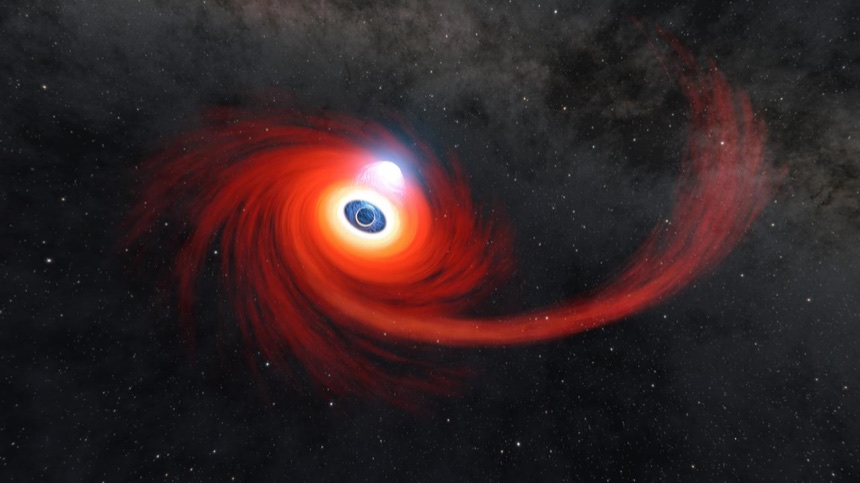
\includegraphics[width=0.78\textwidth,height=5.6cm,keepaspectratio]{../public/textures/nasa/sagittarius_a.jpg}\\[3pt]
{\footnotesize\itshape\color{orbitarMuted} Imaginea istorică reală Event Horizon Telescope (EHT) \& NASA (PIA25440): Gaura neagră supermasivă Sagittarius A* din centrul Căii Lactee.}
\end{center}


\begin{tcolorbox}[orbitardata, title={\textbf{Repere esențiale: Sagittarius A* (Gaura Neagră Supermasivă)}}]
\small
\begin{itemize}[leftmargin=1.4em, itemsep=2pt, topsep=2pt]
  \item \textbf{Clasificare și orbită:} Gaură Neagră Supermasivă \quad$\bullet$\quad \textbf{Distanță:} 26.000 de ani-lumină
  \item \textbf{Dimensiuni și masă:} Orizontul evenimentelor lui Sagittarius A* are diametrul de aproximativ 24 de milioane de kilometri (încape în interiorul orbitei lui Mercur), dar cântărește cât 4,3 milioane de Sori la un loc! \quad$\bullet$\quad masă: 1430000000000,000 $\times M_\oplus$
  \item \textbf{Gravitație și regim termic:} 1000000,000 $\times g_\oplus$ (9810000,00 m/s$^2$) \quad$\bullet$\quad temperatură medie: +1.000.000 $^\circ$C
  \item \textbf{Ciclu orbital și rotație:} perioadă orbitală (an): Orbitează centrul Căii Lactee (aproximativ 230 de milioane de ani) \quad$\bullet$\quad rotație (zi): 1,00 ore (0,04 zile pământești)
  \item \textbf{Durata călătoriei de pe Pământ:} cu viteza luminii ($1c$): \emph{26.000 de ani}; cu racheta ($50.000$ de kilometri pe oră): \emph{468 de milioane de ani}; cu avionul ($900$ de kilometri pe oră): \emph{32.000 de miliarde de ani}; cu mașina ($100$ de kilometri pe oră): \emph{290.000 de miliarde de ani}.
  \item \textbf{Repere de scară și curiozitate:} Sagittarius A* este ca \quotedblbase{}ancora gravitațională\textquotedblright{} din centrul unui carusel gigantic: se află la 26.000 de ani-lumină depărtare, în siguranță totală față de noi, iar întregul Sistem Solar se rotește liniștit în jurul centrului galaxiei o dată la 230 de milioane de ani! În anul 2022, astronomii au unit radiotelescoape de pe tot Pământul (Event Horizon Telescope) și au făcut prima fotografie reală din istorie a inelului portocaliu strălucitor din jurul lui Sagittarius A*!
\end{itemize}
\end{tcolorbox}

\vspace{4pt}
\noindent\textbf{Prezentare generală și profil astrofizic.} Sagittarius A* (Sgr A*), situată la aproximativ 26.000 de ani-lumină în direcția constelației Săgetătorul, este gaura neagră supermasivă din nucleul Căii Lactee. Are o masă de 4,3 milioane de mase solare și o rază Schwarzschild (orizontul evenimentelor, adică limita dincolo de care viteza de evadare depășește viteza luminii) de aproximativ 12 milioane de kilometri. Chiar în mijlocul galaxiei noastre, Calea Lactee, se află un obiect cosmic fascinant: Sagittarius A*, o gaură neagră supermasivă! Nu este o \quotedblbase{}gaură\textquotedblright{} goală, ci un loc în care masa a 4 milioane de Sori este adunată într-un spațiu mic. Gravitația ei este atât de puternică încât înconjoară întunericul central cu un inel luminos și fierbinte de gaz numit \quotedblbase{}disc de acreție\textquotedblright{}, iar lumina din spate este îndoită ca printr-o lupă! Sagittarius A* este ca \quotedblbase{}ancora gravitațională\textquotedblright{} din centrul unui carusel gigantic: se află la 26.000 de ani-lumină depărtare, în siguranță totală față de noi, iar întregul Sistem Solar se rotește liniștit în jurul centrului galaxiei o dată la 230 de milioane de ani!

\medskip
\noindent\textbf{Scara cosmică și călătoria luminii în timp.} La scară astronomică, dimensiunile sale sunt impresionante: Orizontul evenimentelor lui Sagittarius A* are diametrul de aproximativ 24 de milioane de kilometri (încape în interiorul orbitei lui Mercur), dar cântărește cât 4,3 milioane de Sori la un loc! Totodată, privind astăzi spre Sagittarius A* (Gaura Neagră Supermasivă), observăm practic trecutul îndepărtat al Universului, întrucât lumina sa a călătorit prin spațiu până la noi: Lumina discului din jurul găurii negre Sagittarius A* pe care o vedem azi a plecat acum 26.000 de ani, în timpul Epocii de Gheață, când oamenii preistorici pictau peșterile și pe Pământ trăiau mamuții!

\medskip
\noindent\textbf{Alcătuirea fizică și structura internă.} Privind în profunzimea sa, alcătuirea fizică este organizată pe mai multe straturi și regiuni distincte, fiecare având un rol bine definit în evoluția și dinamica acestui obiect cosmic. În primul rând se remarcă \textbf{Orizontul Evenimentelor (Raza Schwarzschild)}, frontiera sferică (aproximativ 12 milioane de kilometri rază) dincolo de care nici măcar fotonii de lumină nu mai pot scăpa de atracția gravitațională. În completarea acestui ansamblu întâlnim \textbf{Discul de Acreție \& Inelul Fotonic}, gaz ionizat rotindu-se la viteze relativiste în jurul găurii negre, a cărui lumină este curbată de lentila gravitațională.

\medskip
\noindent\textbf{Observații astronomice și istoricul explorării.} Existența ei a fost demonstrată prin urmărirea timp de 25 de ani a orbitelor stelelor \quotedblbase{}S\textquotedblright{} (în special steaua S2) de către Reinhard Genzel și Andrea Ghez (Premiul Nobel pentru Fizică 2020), iar în mai 2022 colaborarea Event Horizon Telescope (EHT) a publicat prima imagine directă a umbrei și a inelului său de acreție. În anul 2022, astronomii au unit radiotelescoape de pe tot Pământul (Event Horizon Telescope) și au făcut prima fotografie reală din istorie a inelului portocaliu strălucitor din jurul lui Sagittarius A*!

\vspace{6pt}
\begin{tcolorbox}[orbitarquiz, title={\textbf{Întrebare de verificare \#56: Sagittarius A* (Gaura Neagră Supermasivă)}}]
\textbf{Ce este \quotedblbase{}orizontul evenimentelor\textquotedblright{} al găurii negre Sagittarius A* din centrul Căii Lactee?}
\begin{itemize}[leftmargin=2.2em, itemsep=2pt, topsep=4pt]
  \item[$\square$ \textbf{A.}] Limita în jurul găurii negre dincolo de care gravitația este atât de puternică încât nici lumina nu mai poate ieși
  \item[$\square$ \textbf{B.}] Un lanț de munți de pe planeta Marte
  \item[$\square$ \textbf{C.}] Numele unei sonde spațiale lansate spre Jupiter
  \item[$\square$ \textbf{D.}] Un strat de nori din atmosfera Pământului
\end{itemize}
\vspace{2pt}
{\footnotesize\color{orbitarMuted}\textbf{Răspuns corect:} \textbf{A} (Limita în jurul găurii negre dincolo de care gravitația este atât de puternică încât nici lumina nu mai poate ieși). \emph{Orizontul evenimentelor este granița gravitațională a unei găuri negre unde viteza necesară pentru a scăpa depășește viteza luminii (300.000 kilometri pe secundă).}}
\end{tcolorbox}
\clearpage


\section{Calea Lactee (Galaxia Noastră)}
\label{sec:body-milky_way}
\vspace{-4pt}
{\large\itshape\color{orbitarAccent} Galaxia noastră spirală cu aproximativ 200--400 de miliarde de stele; Soarele se află în Brațul Orion (la 26.000 a.l. de centru)}\\[4pt]


\begin{center}
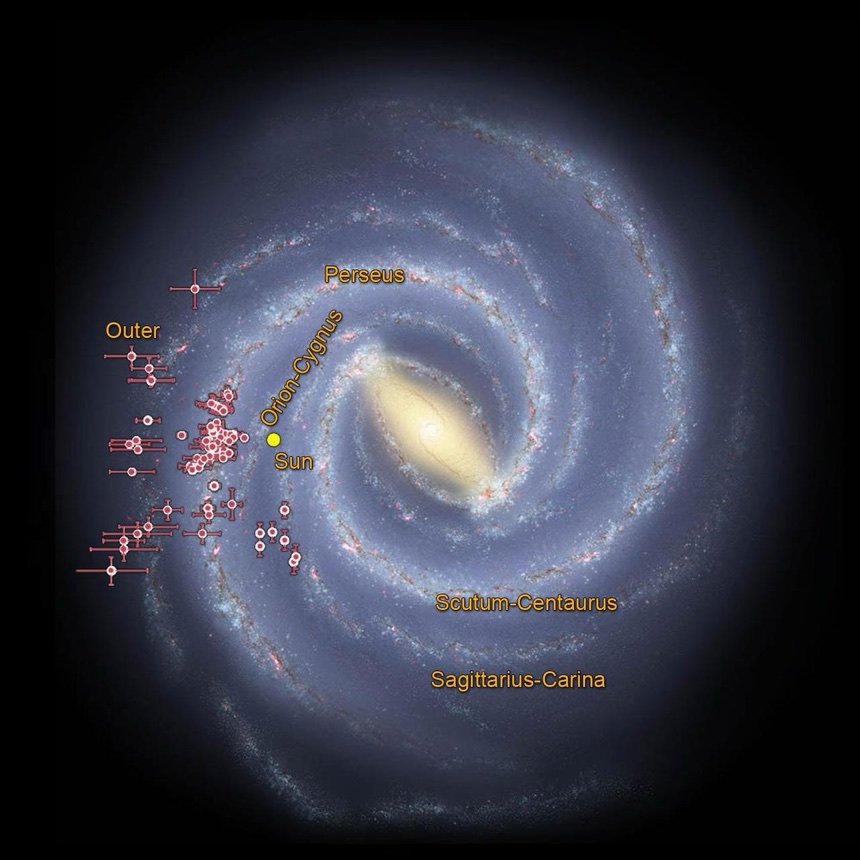
\includegraphics[width=0.78\textwidth,height=5.6cm,keepaspectratio]{../public/textures/nasa/milky_way.jpg}\\[3pt]
{\footnotesize\itshape\color{orbitarMuted} Harta științifică oficială NASA/JPL-Caltech (Telescopul Spitzer PIA19341): Brațele spirale ale galaxiei noastre, Calea Lactee, și poziția Soarelui.}
\end{center}


\begin{tcolorbox}[orbitardata, title={\textbf{Repere esențiale: Calea Lactee (Galaxia Noastră)}}]
\small
\begin{itemize}[leftmargin=1.4em, itemsep=2pt, topsep=2pt]
  \item \textbf{Clasificare și orbită:} Galaxie \quad$\bullet$\quad \textbf{Distanță:} Diametru aproximativ 100.000 ani-lumină (Soarele la 26.000 a.l. de centru)
  \item \textbf{Dimensiuni și masă:} Calea Lactee are un diametru de aproximativ 100.000 de ani-lumină și adăpostește între 200 și 400 de miliarde de stele! Sistemul nostru Solar este doar un punct minuscul în Brațul Orion, la jumătatea distanței dintre centru și margine! \quad$\bullet$\quad masă: 333000000000000000,000 $\times M_\oplus$
  \item \textbf{Gravitație și regim termic:} 1,000 $\times g_\oplus$ (9,81 m/s$^2$) \quad$\bullet$\quad temperatură medie: -270 $^\circ$C
  \item \textbf{Ciclu orbital și rotație:} perioadă orbitală (an): 83.950.000.000 zile ($\approx$ 229842573,58 ani pământești) \quad$\bullet$\quad rotație (zi): 24,00 ore (1,00 zile pământești)
  \item \textbf{Durata călătoriei de pe Pământ:} cu viteza luminii ($1c$): \emph{100.000 de ani (diametrul galaxiei)}; cu racheta ($50.000$ de kilometri pe oră): \emph{1,8 miliarde de ani}; cu avionul ($900$ de kilometri pe oră): \emph{120.000 de miliarde de ani}; cu mașina ($100$ de kilometri pe oră): \emph{1.100.000 de miliarde de ani (de la un capăt la altul)}.
  \item \textbf{Repere de scară și curiozitate:} Dacă întreaga Cale Lactee ar fi cât un stadion mare de fotbal, tot Sistemul nostru Solar (cu Soarele și toate cele 8 planete) ar fi mai mic decât un singur fir de praf așezat pe iarbă, la jumătatea distanței dintre centrul terenului și tribună! Soarele și Pământul călătoresc prin galaxie cu 828.000 kilometri pe oră, dar Calea Lactee este atât de mare încât ne trebuie 230 de milioane de ani ca să facem un singur tur complet (numit \quotedblbase{}un an galactic\textquotedblright{}), astfel că ultima dată când Sistemul Solar s-a aflat în același loc pe orbită, primii dinozauri abia apăreau pe Pământ!
\end{itemize}
\end{tcolorbox}

\vspace{4pt}
\noindent\textbf{Prezentare generală și profil astrofizic.} Calea Lactee este o galaxie spirală barată (tip morfologic SBbc) cu diametrul discului stelar de aproximativ 100.000 de ani-lumină, grosimea de aproximativ 1.000 de ani-lumină și o populație de 200--400 de miliarde de stele. Sistemul Solar este situat în Brațul Local (Orion-Cygnus), la aproximativ 26.000 de ani-lumină de nucleul galactic (Sagittarius A*), orbitând cu aproximativ 220--230 kilometri pe secundă. Calea Lactee este marea noastră casă din Univers, un imens disc cosmic în formă de morișcă spiralată, format din peste 200 de miliarde de stele! Soarele nostru, împreună cu Pământul și toate planetele, locuiește într-un cartier liniștit numit \quotedblbase{}Brațul Orion\textquotedblright{}, la 26.000 de ani-lumină de centrul luminos al galaxiei! Dacă întreaga Cale Lactee ar fi cât un stadion mare de fotbal, tot Sistemul nostru Solar (cu Soarele și toate cele 8 planete) ar fi mai mic decât un singur fir de praf așezat pe iarbă, la jumătatea distanței dintre centrul terenului și tribună!

\medskip
\noindent\textbf{Scara cosmică și călătoria luminii în timp.} La scară astronomică, dimensiunile sale sunt impresionante: Calea Lactee are un diametru de aproximativ 100.000 de ani-lumină și adăpostește între 200 și 400 de miliarde de stele! Sistemul nostru Solar este doar un punct minuscul în Brațul Orion, la jumătatea distanței dintre centru și margine! Totodată, privind astăzi spre Calea Lactee (Galaxia Noastră), observăm practic trecutul îndepărtat al Universului, întrucât lumina sa a călătorit prin spațiu până la noi: Lumina îi ia 100.000 de ani ca să traverseze Calea Lactee de la o margine la cealaltă, iar de la centrul galaxiei până la Pământ călătorește 26.000 de ani!

\medskip
\noindent\textbf{Alcătuirea fizică și structura internă.} Privind în profunzimea sa, alcătuirea fizică este organizată pe mai multe straturi și regiuni distincte, fiecare având un rol bine definit în evoluția și dinamica acestui obiect cosmic. În primul rând se remarcă \textbf{Nucleul Galactic \& Bara Centrală}, regiune centrală densă de stele bătrâne galben-aurii în jurul găurii negre supermasive Sagittarius A*. În strânsă legătură cu această componentă se află \textbf{Brațele Spirale (Perseu, Scutum-Centaurus, Sagittarius, Norma)}, brațe bogate în gaz interstelar, nebuloase și stele tinere albastre fierbinți. În completarea acestui ansamblu întâlnim \textbf{Brațul Orion, Casa Sistemului Solar}, brațul spiral secundar aflat la 26.000 de ani-lumină de centru, unde se găsesc Soarele, Nebuloasa Orion și Pleiadele.

\medskip
\noindent\textbf{Observații astronomice și istoricul explorării.} În 1610, Galileo Galilei a demonstrat cu luneta sa că banda lăptoasă de pe cer este compusă din nenumărate stele; în anii 1920, Harlow Shapley și Edwin Hubble au stabilit dimensiunile galaxiei noastre și existența altor galaxii, iar misiunea europeană Gaia (ESA) a cartografiat recent în 3D aproape 2 miliarde de stele din Calea Lactee. Soarele și Pământul călătoresc prin galaxie cu 828.000 kilometri pe oră, dar Calea Lactee este atât de mare încât ne trebuie 230 de milioane de ani ca să facem un singur tur complet (numit \quotedblbase{}un an galactic\textquotedblright{}), astfel că ultima dată când Sistemul Solar s-a aflat în același loc pe orbită, primii dinozauri abia apăreau pe Pământ!

\vspace{6pt}
\begin{tcolorbox}[orbitarquiz, title={\textbf{Întrebare de verificare \#57: Calea Lactee (Galaxia Noastră)}}]
\textbf{Unde se află Sistemul nostru Solar în cadrul Galaxiei Calea Lactee?}
\begin{itemize}[leftmargin=2.2em, itemsep=2pt, topsep=4pt]
  \item[$\square$ \textbf{A.}] În Brațul Orion, la aproximativ 26.000 de ani-lumină de centrul galaxiei
  \item[$\square$ \textbf{B.}] Chiar în mijlocul găurii negre centrale
  \item[$\square$ \textbf{C.}] În afara galaxiei, lângă Andromeda
  \item[$\square$ \textbf{D.}] Pe suprafața stelei Betelgeuse
\end{itemize}
\vspace{2pt}
{\footnotesize\color{orbitarMuted}\textbf{Răspuns corect:} \textbf{A} (În Brațul Orion, la aproximativ 26.000 de ani-lumină de centrul galaxiei). \emph{Soarele și planetele noastre se află în Brațul Orion, la aproximativ 26.000 de ani-lumină de centrul Căii Lactee (cam la jumătatea razei discului galactic).}}
\end{tcolorbox}
\clearpage


\section{Galaxia Andromeda (M31)}
\label{sec:body-andromeda}
\vspace{-4pt}
{\large\itshape\color{orbitarAccent} Cea mai apropiată galaxie spirală mare, cu aproximativ 1.000 de miliarde de stele (2,5 milioane ani-lumină)}\\[4pt]


\begin{center}
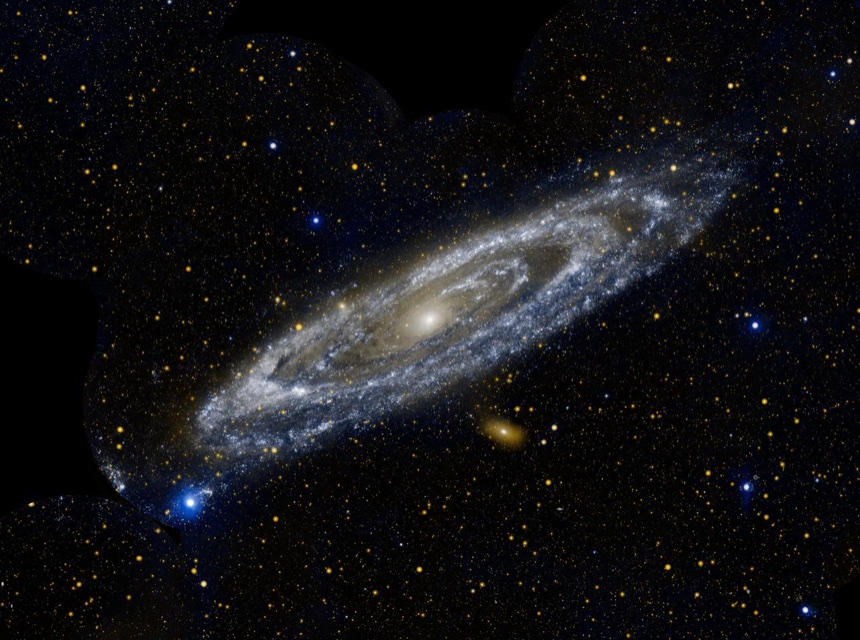
\includegraphics[width=0.78\textwidth,height=5.6cm,keepaspectratio]{../public/textures/nasa/andromeda.jpg}\\[3pt]
{\footnotesize\itshape\color{orbitarMuted} Fotografie reală NASA/JPL-Caltech (GALEX \& Spitzer PIA15416): Galaxia spirală Andromeda (M31), aflată la 2,54 de milioane de ani-lumină.}
\end{center}


\begin{tcolorbox}[orbitardata, title={\textbf{Repere esențiale: Galaxia Andromeda (M31)}}]
\small
\begin{itemize}[leftmargin=1.4em, itemsep=2pt, topsep=2pt]
  \item \textbf{Clasificare și orbită:} Galaxie \quad$\bullet$\quad \textbf{Distanță:} 2,54 de milioane de ani-lumină
  \item \textbf{Dimensiuni și masă:} Galaxia Andromeda are un diametru de aproximativ 150.000--220.000 de ani-lumină și aproximativ 1.000 de miliarde (un bilion) de stele și este chiar mai mare decât Calea Lactee! \quad$\bullet$\quad masă: 500000000000000000,000 $\times M_\oplus$
  \item \textbf{Gravitație și regim termic:} 1,000 $\times g_\oplus$ (9,81 m/s$^2$) \quad$\bullet$\quad temperatură medie: -270 $^\circ$C
  \item \textbf{Ciclu orbital și rotație:} perioadă orbitală (an): Orbitează centrul Căii Lactee (aproximativ 230 de milioane de ani) \quad$\bullet$\quad rotație (zi): 24,00 ore (1,00 zile pământești)
  \item \textbf{Durata călătoriei de pe Pământ:} cu viteza luminii ($1c$): \emph{2,54 de milioane de ani}; cu racheta ($50.000$ de kilometri pe oră): \emph{45 de miliarde de ani}; cu avionul ($900$ de kilometri pe oră): \emph{3,1 milioane de miliarde de ani}; cu mașina ($100$ de kilometri pe oră): \emph{28 de milioane de miliarde de ani}.
  \item \textbf{Repere de scară și curiozitate:} Dacă Calea Lactee ar fi o farfurie mare pe masă, Galaxia Andromeda ar fi o farfurie și mai mare aflată la doar câțiva metri distanță, iar lumina de la ea călătorește spre noi timp de 2,5 milioane de ani! Calea Lactee și Galaxia Andromeda se apropie una de cealaltă cu 400.000 kilometri pe oră! Peste aproximativ 4,5 miliarde de ani, cele două galaxii vor dansa împreună și se vor uni într-o singură galaxie gigantă fără ca stelele să se ciocnească între ele!
\end{itemize}
\end{tcolorbox}

\vspace{4pt}
\noindent\textbf{Prezentare generală și profil astrofizic.} Galaxia Andromeda (Messier 31 / NGC 224), aflată la 2,537 de milioane de ani-lumină în constelația Andromeda, este cea mai mare galaxie din Grupul Local (care include și Calea Lactee și Galaxia Triunghiului M33). Cu un diametru de aproximativ 152.000--220.000 de ani-lumină și aproximativ 10$^1$$^2$ stele, Andromeda a jucat un rol decisiv în istoria științei când Edwin Hubble a demonstrat în 1924 că este o \quotedblbase{}insulă-univers\textquotedblright{} separată de Calea Lactee. Galaxia Andromeda (M31) este \quotedblbase{}sora mai mare\textquotedblright{} a Căii Lactee și cel mai îndepărtat obiect din Univers pe care îl poți vedea cu ochiul liber, fără telescop, într-o noapte senină la munte! Este o galaxie spirală uriașă cu o mie de miliarde de stele, aflată la 2,5 milioane de ani-lumină de noi! Dacă Calea Lactee ar fi o farfurie mare pe masă, Galaxia Andromeda ar fi o farfurie și mai mare aflată la doar câțiva metri distanță, iar lumina de la ea călătorește spre noi timp de 2,5 milioane de ani!

\medskip
\noindent\textbf{Scara cosmică și călătoria luminii în timp.} La scară astronomică, dimensiunile sale sunt impresionante: Galaxia Andromeda are un diametru de aproximativ 150.000--220.000 de ani-lumină și aproximativ 1.000 de miliarde (un bilion) de stele și este chiar mai mare decât Calea Lactee! Totodată, privind astăzi spre Galaxia Andromeda (M31), observăm practic trecutul îndepărtat al Universului, întrucât lumina sa a călătorit prin spațiu până la noi: Lumina de la Galaxia Andromeda pe care o vedem azi cu ochiul liber într-o noapte senină la munte a plecat acum 2,5 milioane de ani, de la începutul Cuaternarului, cu mult înainte să apară omul modern (Homo sapiens) pe Pământ!

\medskip
\noindent\textbf{Alcătuirea fizică și structura internă.} Privind în profunzimea sa, alcătuirea fizică este organizată pe mai multe straturi și regiuni distincte, fiecare având un rol bine definit în evoluția și dinamica acestui obiect cosmic. În primul rând se remarcă \textbf{Nucleu Dublu \& Gaură Neagră de aproximativ 100 Milioane M$_\odot$}, centru galactic masiv observat de telescopul Hubble, multă vreme mai masiv decât nucleul Căii Lactee. În completarea acestui ansamblu întâlnim \textbf{Discul Spiral și Galaxiile Satelit (M32 \& M110)}, brațe spirale bogate în roiuri stelare și praf, însoțite de galaxiile pitice eliptice M32 și M110.

\medskip
\noindent\textbf{Observații astronomice și istoricul explorării.} Menționată în anul 964 de astronomul persan Abd al-Rahman al-Sufi drept \quotedblbase{}un mic nor\textquotedblright{}; în 1924, Edwin Hubble a identificat stele variabile Cefeide în M31, demonstrând că Universul se întinde mult dincolo de Calea Lactee. Calea Lactee și Galaxia Andromeda se apropie una de cealaltă cu 400.000 kilometri pe oră! Peste aproximativ 4,5 miliarde de ani, cele două galaxii vor dansa împreună și se vor uni într-o singură galaxie gigantă fără ca stelele să se ciocnească între ele!

\vspace{6pt}
\begin{tcolorbox}[orbitarquiz, title={\textbf{Întrebare de verificare \#58: Galaxia Andromeda (M31)}}]
\textbf{Care este cel mai îndepărtat obiect cosmic vizibil cu ochiul liber pe cerul nopții și la ce distanță se află?}
\begin{itemize}[leftmargin=2.2em, itemsep=2pt, topsep=4pt]
  \item[$\square$ \textbf{A.}] Galaxia Andromeda (M31), aflată la aproximativ 2,5 milioane de ani-lumină
  \item[$\square$ \textbf{B.}] Planeta Neptun, la 4 ore-lumină
  \item[$\square$ \textbf{C.}] Luna, la 1,3 secunde-lumină
  \item[$\square$ \textbf{D.}] Sonda Voyager 1, la 22 ore-lumină
\end{itemize}
\vspace{2pt}
{\footnotesize\color{orbitarMuted}\textbf{Răspuns corect:} \textbf{A} (Galaxia Andromeda (M31), aflată la aproximativ 2,5 milioane de ani-lumină). \emph{Galaxia Andromeda (M31), situată la 2,54 de milioane de ani-lumină, poate fi văzută cu ochiul liber într-o noapte fără poluare luminoasă.}}
\end{tcolorbox}
\clearpage


\section{Nebuloasa Carina (\quotedblbase{}Stâncile Cosmice\textquotedblright{}, NGC 3372)}
\label{sec:body-carina_nebula}
\vspace{-4pt}
{\large\itshape\color{orbitarAccent} Una dintre cele mai mari maternități de stele din Calea Lactee, fotografiată de James Webb (7.500 ani-lumină)}\\[4pt]



\begin{tcolorbox}[orbitardata, title={\textbf{Repere esențiale: Nebuloasa Carina (\quotedblbase{}Stâncile Cosmice\textquotedblright{}, NGC 3372)}}]
\small
\begin{itemize}[leftmargin=1.4em, itemsep=2pt, topsep=2pt]
  \item \textbf{Clasificare și orbită:} Nebuloasă Cosmică \quad$\bullet$\quad \textbf{Distanță:} 7.500 de ani-lumină
  \item \textbf{Dimensiuni și masă:} Nebuloasa Carina se întinde pe aproximativ 300 de ani-lumină și este de peste 10 ori mai mare decât Nebuloasa Orion! \quad$\bullet$\quad masă: 300000000,000 $\times M_\oplus$
  \item \textbf{Gravitație și regim termic:} 0,100 $\times g_\oplus$ (0,98 m/s$^2$) \quad$\bullet$\quad temperatură medie: +9.500 $^\circ$C
  \item \textbf{Ciclu orbital și rotație:} perioadă orbitală (an): Orbitează centrul Căii Lactee (aproximativ 230 de milioane de ani) \quad$\bullet$\quad rotație (zi): 24,00 ore (1,00 zile pământești)
  \item \textbf{Durata călătoriei de pe Pământ:} cu viteza luminii ($1c$): \emph{7.500 de ani}; cu racheta ($50.000$ de kilometri pe oră): \emph{135 de milioane de ani}; cu avionul ($900$ de kilometri pe oră): \emph{9.300 de miliarde de ani}; cu mașina ($100$ de kilometri pe oră): \emph{84.000 de miliarde de ani}.
  \item \textbf{Repere de scară și curiozitate:} Nebuloasa Carina arată ca un lanț muntos de chihlimbar scăldat de un cer azuriu, doar că \quotedblbase{}munții\textquotedblright{} sunt făcuți din nori de praf stelar mai înalți decât distanța de la Soare la cea mai apropiată stea! În inima Nebuloasei Carina locuiește Eta Carinae, un sistem de două stele monstruoase care luminează cât 5 milioane de Sori la un loc!
\end{itemize}
\end{tcolorbox}

\vspace{4pt}
\noindent\textbf{Prezentare generală și profil astrofizic.} Nebuloasa Carina (NGC 3372), situată la aproximativ 7.500 de ani-lumină în Brațul Carina-Sagittarius al Căii Lactee, este una dintre cele mai întinse regiuni H II din galaxia noastră (aproximativ 300 ani-lumină diametru). Pe marginea cavității NGC 3324 se ridică \quotedblbase{}Stâncile Cosmice\textquotedblright{}, sculptate de vânturile stelare și radiația ultravioletă a stelelor masive tinere de tip O. Nebuloasa Carina este un ținut cosmic uriaș, unde munți înalți de gaz și praf portocaliu se întâlnesc cu o mare strălucitoare de lumină albastră! Prima fotografie celebră trimisă de Telescopul Spațial James Webb ne-a arătat aici \quotedblbase{}Stâncile Cosmice\textquotedblright{}, creste înalte de 7 ani-lumină în care se aprind mii de stele noi! Nebuloasa Carina arată ca un lanț muntos de chihlimbar scăldat de un cer azuriu, doar că \quotedblbase{}munții\textquotedblright{} sunt făcuți din nori de praf stelar mai înalți decât distanța de la Soare la cea mai apropiată stea!

\medskip
\noindent\textbf{Scara cosmică și călătoria luminii în timp.} La scară astronomică, dimensiunile sale sunt impresionante: Nebuloasa Carina se întinde pe aproximativ 300 de ani-lumină și este de peste 10 ori mai mare decât Nebuloasa Orion! Totodată, privind astăzi spre Nebuloasa Carina (\quotedblbase{}Stâncile Cosmice\textquotedblright{}, NGC 3372), observăm practic trecutul îndepărtat al Universului, întrucât lumina sa a călătorit prin spațiu până la noi: Lumina de la Stâncile Cosmice din Nebuloasa Carina a plecat spre Pământ acum 7.500 de ani (în jurul anului 5500 î.Hr.), la începutul Neoliticului!

\medskip
\noindent\textbf{Alcătuirea fizică și structura internă.} Privind în profunzimea sa, alcătuirea fizică este organizată pe mai multe straturi și regiuni distincte, fiecare având un rol bine definit în evoluția și dinamica acestui obiect cosmic. În primul rând se remarcă \textbf{Stâncile Cosmice (NGC 3324)}, front de gaz și praf înalt de aproximativ 7 ani-lumină, modelat de radiația ionizantă și străbătut de jeturi protostelare. În completarea acestui ansamblu întâlnim \textbf{Sistemul Hipergigant Eta Carinae \& Nebuloasa Homunculus}, stea variabilă luminoasă albastră (aproximativ 100 mase solare) înconjurată de doi lobi bipolari de gaz expulzați în Marea Erupție din 1843.

\medskip
\noindent\textbf{Observații astronomice și istoricul explorării.} Descoperită în 1752 de Nicolas-Louis de Lacaille de la Capul Bunei Speranțe; în iulie 2022, \quotedblbase{}Stâncile Cosmice\textquotedblright{} au devenit una dintre primele imagini istorice publicate de Telescopul Spațial James Webb. În inima Nebuloasei Carina locuiește Eta Carinae, un sistem de două stele monstruoase care luminează cât 5 milioane de Sori la un loc!

\vspace{6pt}
\begin{tcolorbox}[orbitarquiz, title={\textbf{Întrebare de verificare \#59: Nebuloasa Carina (\quotedblbase{}Stâncile Cosmice\textquotedblright{}, NGC 3372)}}]
\textbf{Cum se numește formațiunea spectaculoasă din Nebuloasa Carina fotografiată în prima serie de imagini a Telescopului James Webb?}
\begin{itemize}[leftmargin=2.2em, itemsep=2pt, topsep=4pt]
  \item[$\square$ \textbf{A.}] Stâncile Cosmice, creste de gaz și praf înalte de 7 ani-lumină unde se nasc stele
  \item[$\square$ \textbf{B.}] Inelul lui Saturn
  \item[$\square$ \textbf{C.}] Craterul Tycho de pe Lună
  \item[$\square$ \textbf{D.}] Marea Pată Roșie de pe Jupiter
\end{itemize}
\vspace{2pt}
{\footnotesize\color{orbitarMuted}\textbf{Răspuns corect:} \textbf{A} (Stâncile Cosmice, creste de gaz și praf înalte de 7 ani-lumină unde se nasc stele). \emph{\quotedblbase{}Stâncile Cosmice\textquotedblright{} din NGC 3324 (Nebuloasa Carina) reprezintă marginea unei cavități gazoase uriașe sculptate de stele tinere masive.}}
\end{tcolorbox}
\clearpage


\section{Nebuloasa Crabului (M1)}
\label{sec:body-crab_nebula}
\vspace{-4pt}
{\large\itshape\color{orbitarAccent} Rămășița luminoasă a supernovei observate în anul 1054, cu un pulsar în centru (6.500 ani-lumină)}\\[4pt]



\begin{tcolorbox}[orbitardata, title={\textbf{Repere esențiale: Nebuloasa Crabului (M1)}}]
\small
\begin{itemize}[leftmargin=1.4em, itemsep=2pt, topsep=2pt]
  \item \textbf{Clasificare și orbită:} Nebuloasă Cosmică \quad$\bullet$\quad \textbf{Distanță:} 6.500 de ani-lumină
  \item \textbf{Dimensiuni și masă:} Nebuloasa Crabului are un diametru de 11 ani-lumină și încă se mărește în fiecare secundă cu 1.500 kilometri pe secundă! \quad$\bullet$\quad masă: 1500000,000 $\times M_\oplus$
  \item \textbf{Gravitație și regim termic:} 1,000 $\times g_\oplus$ (9,81 m/s$^2$) \quad$\bullet$\quad temperatură medie: +15.000 $^\circ$C
  \item \textbf{Ciclu orbital și rotație:} perioadă orbitală (an): Orbitează centrul Căii Lactee (aproximativ 230 de milioane de ani) \quad$\bullet$\quad rotație (zi): 0,00 ore (0,00 zile pământești)
  \item \textbf{Durata călătoriei de pe Pământ:} cu viteza luminii ($1c$): \emph{6.500 de ani}; cu racheta ($50.000$ de kilometri pe oră): \emph{117 milioane de ani}; cu avionul ($900$ de kilometri pe oră): \emph{8.100 de miliarde de ani}; cu mașina ($100$ de kilometri pe oră): \emph{73.000 de miliarde de ani}.
  \item \textbf{Repere de scară și curiozitate:} În mijlocul Nebuloasei Crabului se află \quotedblbase{}inima\textquotedblright{} stelei care a explodat: o stea neutronică mică doar cât un oraș (25 de kilometri), dar care se învârte ca un titirez de 30 de ori pe secundă și trimite fascicule de lumină ca un far cosmic! Nebuloasa Crabului este primul obiect trecut în faimosul catalog al astronomului Charles Messier, motiv pentru care poartă numele \quotedblbase{}M1\textquotedblright{} (Messier 1)!
\end{itemize}
\end{tcolorbox}

\vspace{4pt}
\noindent\textbf{Prezentare generală și profil astrofizic.} Nebuloasa Crabului (Messier 1 / NGC 1952), situată la 6.500 de ani-lumină în constelația Taurul, este o rămășiță de supernovă și o nebuloasă de vânt pulsaric alimentată de Pulsarul din Crab (PSR B0531+21). Steaua neutronică centrală se rotește la fiecare 33 de milisecunde (aproximativ 30 rotații pe secundă), accelerând electroni la viteze relativiste care emit radiație sincrotron albăstruie. În anul 1054, oamenii de pe Pământ au văzut pe cer o \quotedblbase{}stea nouă\textquotedblright{} atât de strălucitoare încât se vedea chiar și ziua, în plin soare! Era explozia unei stele uriașe (o supernovă), iar norul țesut din filamente colorate rămas în urma ei se numește azi Nebuloasa Crabului! În mijlocul Nebuloasei Crabului se află \quotedblbase{}inima\textquotedblright{} stelei care a explodat: o stea neutronică mică doar cât un oraș (25 de kilometri), dar care se învârte ca un titirez de 30 de ori pe secundă și trimite fascicule de lumină ca un far cosmic!

\medskip
\noindent\textbf{Scara cosmică și călătoria luminii în timp.} La scară astronomică, dimensiunile sale sunt impresionante: Nebuloasa Crabului are un diametru de 11 ani-lumină și încă se mărește în fiecare secundă cu 1.500 kilometri pe secundă! Totodată, privind astăzi spre Nebuloasa Crabului (M1), observăm practic trecutul îndepărtat al Universului, întrucât lumina sa a călătorit prin spațiu până la noi: Explozia stelei a fost văzută pe cerul Pământului în anul 1054 d.Hr., dar lumina acelei explozii plecase din Nebuloasa Crabului cu 6.500 de ani mai devreme!

\medskip
\noindent\textbf{Alcătuirea fizică și structura internă.} Privind în profunzimea sa, alcătuirea fizică este organizată pe mai multe straturi și regiuni distincte, fiecare având un rol bine definit în evoluția și dinamica acestui obiect cosmic. În primul rând se remarcă \textbf{Pulsarul din Crab (Stea Neutronică)}, nucleu stelar colapsat cu diametrul de aproximativ 25 de kilometri și masa de 1,4 Sori, care se rotește de 30 de ori pe secundă. În completarea acestui ansamblu întâlnim \textbf{Cușca de Filamente și Nebuloasa Sincrotron}, rețea tridimensională de filamente bogate în heliu, carbon, oxigen și sulf ce se extinde cu aproximativ 1.500 kilometri pe secundă.

\medskip
\noindent\textbf{Observații astronomice și istoricul explorării.} Supernova SN 1054 a fost consemnată de astronomii chinezi și arabi în iulie 1054; nebuloasa a fost redescoperită în 1731 de John Bevis și catalogată drept M1 de Charles Messier în 1758. Nebuloasa Crabului este primul obiect trecut în faimosul catalog al astronomului Charles Messier, motiv pentru care poartă numele \quotedblbase{}M1\textquotedblright{} (Messier 1)!

\vspace{6pt}
\begin{tcolorbox}[orbitarquiz, title={\textbf{Întrebare de verificare \#60: Nebuloasa Crabului (M1)}}]
\textbf{Ce obiect extraordinar se află chiar în centrul Nebuloasei Crabului (M1)?}
\begin{itemize}[leftmargin=2.2em, itemsep=2pt, topsep=4pt]
  \item[$\square$ \textbf{A.}] Un pulsar (o stea neutronică densă cât un oraș) care se rotește de 30 de ori pe secundă
  \item[$\square$ \textbf{B.}] O planetă acoperită cu păduri tropicale
  \item[$\square$ \textbf{C.}] Un satelit natural al planetei Neptun
  \item[$\square$ \textbf{D.}] O cometă de gheață din Norul lui Oort
\end{itemize}
\vspace{2pt}
{\footnotesize\color{orbitarMuted}\textbf{Răspuns corect:} \textbf{A} (Un pulsar (o stea neutronică densă cât un oraș) care se rotește de 30 de ori pe secundă). \emph{În centrul Nebuloasei Crabului se află Pulsarul din Crab, o stea neutronică rămasă după supernova din anul 1054.}}
\end{tcolorbox}
\clearpage


\section{Nebuloasa Inelul (M57)}
\label{sec:body-ring_nebula}
\vspace{-4pt}
{\large\itshape\color{orbitarAccent} Inelul cosmic în culorile curcubeului lăsat în urmă de o stea asemănătoare Soarelui (2.300 ani-lumină)}\\[4pt]



\begin{tcolorbox}[orbitardata, title={\textbf{Repere esențiale: Nebuloasa Inelul (M57)}}]
\small
\begin{itemize}[leftmargin=1.4em, itemsep=2pt, topsep=2pt]
  \item \textbf{Clasificare și orbită:} Nebuloasă Cosmică \quad$\bullet$\quad \textbf{Distanță:} 2.300 de ani-lumină
  \item \textbf{Dimensiuni și masă:} Inelul luminos principal are un diametru de aproximativ 1,3 ani-lumină, fiind de peste 400 de ori mai lat decât orbita planetei Neptun în jurul Soarelui! \quad$\bullet$\quad masă: 200000,000 $\times M_\oplus$
  \item \textbf{Gravitație și regim termic:} 0,500 $\times g_\oplus$ (4,91 m/s$^2$) \quad$\bullet$\quad temperatură medie: +100.000 $^\circ$C
  \item \textbf{Ciclu orbital și rotație:} perioadă orbitală (an): Orbitează centrul Căii Lactee (aproximativ 230 de milioane de ani) \quad$\bullet$\quad rotație (zi): 24,00 ore (1,00 zile pământești)
  \item \textbf{Durata călătoriei de pe Pământ:} cu viteza luminii ($1c$): \emph{2.300 de ani}; cu racheta ($50.000$ de kilometri pe oră): \emph{41 de milioane de ani}; cu avionul ($900$ de kilometri pe oră): \emph{2.850 de miliarde de ani}; cu mașina ($100$ de kilometri pe oră): \emph{26.000 de miliarde de ani}.
  \item \textbf{Repere de scară și curiozitate:} În mijlocul inelului colorat se vede un punctuleț alb ca o perlă: este o \quotedblbase{}pitică albă\textquotedblright{}, adică miezul cald al stelei, de mărimea Pământului, care luminează gazul din jur ca o lampă cosmică! Telescopul James Webb a descoperit că în jurul inelului se află 20.000 de globuri dense de gaz și zece arce concentrice, ca valurile lăsate de o pietricică într-un lac!
\end{itemize}
\end{tcolorbox}

\vspace{4pt}
\noindent\textbf{Prezentare generală și profil astrofizic.} Nebuloasa Inelul (Messier 57 / NGC 6720), aflată la aproximativ 2.300 de ani-lumină în constelația Lira, este o nebuloasă planetară arhetipală. Deși văzută dinspre Pământ pare un inel, observațiile Hubble și JWST arată că are forma unui cilindru/butoi de gaz ionizat văzut aproape de-a lungul axei polare, iluminat de o pitică albă centrală cu temperatura de aproximativ 120.000 $^\circ$C. Nebuloasa Inelul (M57) arată ca o gogoașă sau un inel fermecat în culorile curcubeului care plutește în spațiu: albastru în interior, verde-turcoaz la mijloc și roșu-auriu pe margine! Ea nu s-a format dintr-o explozie violentă, ci atunci când o stea bătrână, asemănătoare Soarelui nostru, și-a suflat ușor straturile exterioare în spațiu! În mijlocul inelului colorat se vede un punctuleț alb ca o perlă: este o \quotedblbase{}pitică albă\textquotedblright{}, adică miezul cald al stelei, de mărimea Pământului, care luminează gazul din jur ca o lampă cosmică!

\medskip
\noindent\textbf{Scara cosmică și călătoria luminii în timp.} La scară astronomică, dimensiunile sale sunt impresionante: Inelul luminos principal are un diametru de aproximativ 1,3 ani-lumină, fiind de peste 400 de ori mai lat decât orbita planetei Neptun în jurul Soarelui! Totodată, privind astăzi spre Nebuloasa Inelul (M57), observăm practic trecutul îndepărtat al Universului, întrucât lumina sa a călătorit prin spațiu până la noi: Lumina de la Nebuloasa Inelul pe care o admirăm azi a plecat spre noi acum 2.300 de ani, pe vremea vechilor daci și a marelui matematician Arhimede!

\medskip
\noindent\textbf{Alcătuirea fizică și structura internă.} Privind în profunzimea sa, alcătuirea fizică este organizată pe mai multe straturi și regiuni distincte, fiecare având un rol bine definit în evoluția și dinamica acestui obiect cosmic. În primul rând se remarcă \textbf{Pitica Albă Centrală}, nucleul stelar rezidual (0,6 mase solare, de dimensiunea Pământului), extrem de fierbinte în radiație ultravioletă. În completarea acestui ansamblu întâlnim \textbf{Torusul Ionizat \& Haloul Exterior cu Spiculi}, heliu albastru în centru, oxigen dublu ionizat verde-turcoaz în inel și hidrogen/azot roșu pe marginea exterioară.

\medskip
\noindent\textbf{Observații astronomice și istoricul explorării.} Descoperită în ianuarie 1779 de astronomii francezi Antoine Darquier de Pellepoix și Charles Messier; fotografiată la rezoluție fără precedent de JWST în august 2023. Telescopul James Webb a descoperit că în jurul inelului se află 20.000 de globuri dense de gaz și zece arce concentrice, ca valurile lăsate de o pietricică într-un lac!

\vspace{6pt}
\begin{tcolorbox}[orbitarquiz, title={\textbf{Întrebare de verificare \#61: Nebuloasa Inelul (M57)}}]
\textbf{Cum ia naștere o \quotedblbase{}nebuloasă planetară\textquotedblright{} precum Nebuloasa Inelul (M57)?}
\begin{itemize}[leftmargin=2.2em, itemsep=2pt, topsep=4pt]
  \item[$\square$ \textbf{A.}] O stea de mărime medie (ca Soarele) își eliberează straturile exterioare de gaz la finalul vieții, lăsând în centru o pitică albă
  \item[$\square$ \textbf{B.}] Două planete stâncoase se ciocnesc în Centura de Asteroizi
  \item[$\square$ \textbf{C.}] Un vulcan erupe pe satelitul Io
  \item[$\square$ \textbf{D.}] O rachetă spațială pornește motoarele pe orbita Lunii
\end{itemize}
\vspace{2pt}
{\footnotesize\color{orbitarMuted}\textbf{Răspuns corect:} \textbf{A} (O stea de mărime medie (ca Soarele) își eliberează straturile exterioare de gaz la finalul vieții, lăsând în centru o pitică albă). \emph{Nebuloasele planetare sunt învelișuri strălucitoare de gaz expulzate de stele de masă mică și medie, iluminate de pitica albă rămasă în centru.}}
\end{tcolorbox}
\clearpage


\section{Nebuloasa Helix (\quotedblbase{}Ochiul lui Dumnezeu\textquotedblright{}, NGC 7293)}
\label{sec:body-helix_nebula}
\vspace{-4pt}
{\large\itshape\color{orbitarAccent} Cea mai apropiată nebuloasă planetară mare, cu mii de \quotedblbase{}noduri cometare\textquotedblright{} (650 ani-lumină)}\\[4pt]



\begin{tcolorbox}[orbitardata, title={\textbf{Repere esențiale: Nebuloasa Helix (\quotedblbase{}Ochiul lui Dumnezeu\textquotedblright{}, NGC 7293)}}]
\small
\begin{itemize}[leftmargin=1.4em, itemsep=2pt, topsep=2pt]
  \item \textbf{Clasificare și orbită:} Nebuloasă Cosmică \quad$\bullet$\quad \textbf{Distanță:} 650 de ani-lumină
  \item \textbf{Dimensiuni și masă:} Nebuloasa Helix are un diametru de aproximativ 2,8 ani-lumină (cu haloul exterior ajungând la aproape 6 ani-lumină)! \quad$\bullet$\quad masă: 250000,000 $\times M_\oplus$
  \item \textbf{Gravitație și regim termic:} 0,400 $\times g_\oplus$ (3,92 m/s$^2$) \quad$\bullet$\quad temperatură medie: +110.000 $^\circ$C
  \item \textbf{Ciclu orbital și rotație:} perioadă orbitală (an): Orbitează centrul Căii Lactee (aproximativ 230 de milioane de ani) \quad$\bullet$\quad rotație (zi): 24,00 ore (1,00 zile pământești)
  \item \textbf{Durata călătoriei de pe Pământ:} cu viteza luminii ($1c$): \emph{650 de ani}; cu racheta ($50.000$ de kilometri pe oră): \emph{11,7 milioane de ani}; cu avionul ($900$ de kilometri pe oră): \emph{810 miliarde de ani}; cu mașina ($100$ de kilometri pe oră): \emph{7.300 de miliarde de ani}.
  \item \textbf{Repere de scară și curiozitate:} În interiorul acestui \quotedblbase{}ochi\textquotedblright{} uriaș plutesc peste 40.000 de nori rotunzi cu cozi lungi (\quotedblbase{}noduri cometare\textquotedblright{}), fiecare dintre ei fiind mai mare decât tot Sistemul nostru Solar până la Pluto! Peste aproximativ 5 miliarde de ani, și Soarele nostru va crea o nebuloasă colorată foarte asemănătoare cu Nebuloasa Helix!
\end{itemize}
\end{tcolorbox}

\vspace{4pt}
\noindent\textbf{Prezentare generală și profil astrofizic.} Nebuloasa Helix (NGC 7293 / Caldwell 63), situată la 650 de ani-lumină în constelația Vărsătorul, este una dintre cele mai apropiate și mai studiate nebuloase planetare. Structura ei elicoidală dublă conține aproximativ 40.000 de noduri cometare, care sunt condensări dense de gaz molecular ale căror cozi radiale sunt modelate de vântul stelar al piticei albe centrale. Privită prin telescoapele mari, Nebuloasa Helix seamănă atât de mult cu un iris albastru-turcoaz înconjurat de gene roșii-aurii încât astronomii i-au pus porecla \quotedblbase{}Ochiul Cosmic\textquotedblright{} sau \quotedblbase{}Ochiul lui Dumnezeu\textquotedblright{}! Este una dintre cele mai apropiate nebuloase planetare față de Pământ, aflată la doar 650 de ani-lumină! În interiorul acestui \quotedblbase{}ochi\textquotedblright{} uriaș plutesc peste 40.000 de nori rotunzi cu cozi lungi (\quotedblbase{}noduri cometare\textquotedblright{}), fiecare dintre ei fiind mai mare decât tot Sistemul nostru Solar până la Pluto!

\medskip
\noindent\textbf{Scara cosmică și călătoria luminii în timp.} La scară astronomică, dimensiunile sale sunt impresionante: Nebuloasa Helix are un diametru de aproximativ 2,8 ani-lumină (cu haloul exterior ajungând la aproape 6 ani-lumină)! Totodată, privind astăzi spre Nebuloasa Helix (\quotedblbase{}Ochiul lui Dumnezeu\textquotedblright{}, NGC 7293), observăm practic trecutul îndepărtat al Universului, întrucât lumina sa a călătorit prin spațiu până la noi: Lumina de la Nebuloasa Helix a plecat spre Pământ acum 650 de ani (în jurul anului 1375), chiar în perioada în care se întemeiau Țara Românească și Moldova!

\medskip
\noindent\textbf{Alcătuirea fizică și structura internă.} Privind în profunzimea sa, alcătuirea fizică este organizată pe mai multe straturi și regiuni distincte, fiecare având un rol bine definit în evoluția și dinamica acestui obiect cosmic. În primul rând se remarcă \textbf{Cavitatea Interioară \& Pitica Albă}, sferă centrală de gaz foarte fierbinte care emite în ultraviolet și raze X în jurul nucleului stelar. În completarea acestui ansamblu întâlnim \textbf{Cele 40.000 de Noduri Cometare}, globule de gaz cu diametrul comparabil cu Sistemul Solar, având cozi îndreptate opus față de pitica albă.

\medskip
\noindent\textbf{Observații astronomice și istoricul explorării.} Descoperită de astronomul german Karl Ludwig Harding înainte de 1824; studiată în detaliu de telescoapele Hubble, Spitzer și Euclid. Peste aproximativ 5 miliarde de ani, și Soarele nostru va crea o nebuloasă colorată foarte asemănătoare cu Nebuloasa Helix!

\vspace{6pt}
\begin{tcolorbox}[orbitarquiz, title={\textbf{Întrebare de verificare \#62: Nebuloasa Helix (\quotedblbase{}Ochiul lui Dumnezeu\textquotedblright{}, NGC 7293)}}]
\textbf{De ce este supranumită Nebuloasa Helix (NGC 7293) \quotedblbase{}Ochiul Cosmic\textquotedblright{}?}
\begin{itemize}[leftmargin=2.2em, itemsep=2pt, topsep=4pt]
  \item[$\square$ \textbf{A.}] Deoarece inelul ei dublu de gaz turcoaz și roșu-auriu, cu pitica albă în mijloc, seamănă cu irisul și pupila unui ochi
  \item[$\square$ \textbf{B.}] Pentru că este o lentilă de sticlă trimisă în spațiu
  \item[$\square$ \textbf{C.}] Pentru că se află pe suprafața planetei Jupiter
  \item[$\square$ \textbf{D.}] Pentru că se rotește în jurul Lunii
\end{itemize}
\vspace{2pt}
{\footnotesize\color{orbitarMuted}\textbf{Răspuns corect:} \textbf{A} (Deoarece inelul ei dublu de gaz turcoaz și roșu-auriu, cu pitica albă în mijloc, seamănă cu irisul și pupila unui ochi). \emph{Privită de-a lungul axei sale cilindrice, cavitatea albastră-turcoaz și inelul exterior roșiatic al Nebuloasei Helix creează aspectul spectaculos al unui ochi cosmic.}}
\end{tcolorbox}
\clearpage


\section{Marele Nor al lui Magellan}
\label{sec:body-large_magellanic_cloud}
\vspace{-4pt}
{\large\itshape\color{orbitarAccent} Cea mai mare galaxie-satelit luminoasă a Căii Lactee și casa Nebuloasei Tarantula (160.000 ani-lumină)}\\[4pt]



\begin{tcolorbox}[orbitardata, title={\textbf{Repere esențiale: Marele Nor al lui Magellan}}]
\small
\begin{itemize}[leftmargin=1.4em, itemsep=2pt, topsep=2pt]
  \item \textbf{Clasificare și orbită:} Galaxie \quad$\bullet$\quad \textbf{Distanță:} 160.000 de ani-lumină
  \item \textbf{Dimensiuni și masă:} Marele Nor al lui Magellan are un diametru de aproximativ 32.000 de ani-lumină și conține aproximativ 20--30 de miliarde de stele! \quad$\bullet$\quad masă: 3300000000000000,000 $\times M_\oplus$
  \item \textbf{Gravitație și regim termic:} 0,600 $\times g_\oplus$ (5,89 m/s$^2$) \quad$\bullet$\quad temperatură medie: -268 $^\circ$C
  \item \textbf{Ciclu orbital și rotație:} perioadă orbitală (an): Orbitează centrul Căii Lactee (aproximativ 230 de milioane de ani) \quad$\bullet$\quad rotație (zi): 24,00 ore (1,00 zile pământești)
  \item \textbf{Durata călătoriei de pe Pământ:} cu viteza luminii ($1c$): \emph{160.000 de ani}; cu racheta ($50.000$ de kilometri pe oră): \emph{2,9 miliarde de ani}; cu avionul ($900$ de kilometri pe oră): \emph{200.000 de miliarde de ani}; cu mașina ($100$ de kilometri pe oră): \emph{1,8 milioane de miliarde de ani}.
  \item \textbf{Repere de scară și curiozitate:} În interiorul Marelui Nor al lui Magellan se află \quotedblbase{}Nebuloasa Tarantula\textquotedblright{}, o maternitate de stele atât de strălucitoare încât, dacă ar fi la fel de aproape de noi ca Nebuloasa Orion, ar lumina noaptea pe Pământ atât de tare încât copacii ar lăsa umbre! A primit numele navigatorului Fernando Magellan, ale cărui corăbii au văzut acest nor luminos pe cerul sudic în timpul primei călătorii în jurul Pământului (1519--1522)!
\end{itemize}
\end{tcolorbox}

\vspace{4pt}
\noindent\textbf{Prezentare generală și profil astrofizic.} Marele Nor al lui Magellan (LMC), situat la aproximativ 160.000 de ani-lumină pe cerul emisferei sudice (constelațiile Dorado și Mensa), este o galaxie pitică spirală barată neregulată, satelită a Căii Lactee. Găzduiește Nebuloasa Tarantula (30 Doradus, cea mai activă regiune de formare stelară din Grupul Local) și locul celebrei supernove SN 1987A. Așa cum Luna se învârte în jurul Pământului, și galaxia noastră Calea Lactee are propriii ei \quotedblbase{}sateliți\textquotedblright{}, adică galaxii mai mici care o însoțesc prin Univers! Cea mai vestită dintre ele este Marele Nor al lui Magellan, o galaxie tânără și plină de culoare care conține peste 20 de miliarde de stele! În interiorul Marelui Nor al lui Magellan se află \quotedblbase{}Nebuloasa Tarantula\textquotedblright{}, o maternitate de stele atât de strălucitoare încât, dacă ar fi la fel de aproape de noi ca Nebuloasa Orion, ar lumina noaptea pe Pământ atât de tare încât copacii ar lăsa umbre!

\medskip
\noindent\textbf{Scara cosmică și călătoria luminii în timp.} La scară astronomică, dimensiunile sale sunt impresionante: Marele Nor al lui Magellan are un diametru de aproximativ 32.000 de ani-lumină și conține aproximativ 20--30 de miliarde de stele! Totodată, privind astăzi spre Marele Nor al lui Magellan, observăm practic trecutul îndepărtat al Universului, întrucât lumina sa a călătorit prin spațiu până la noi: Lumina de la Marele Nor al lui Magellan a plecat spre noi acum 160.000 de ani, pe vremea când primii oameni moderni trăiau în Africa!

\medskip
\noindent\textbf{Alcătuirea fizică și structura internă.} Privind în profunzimea sa, alcătuirea fizică este organizată pe mai multe straturi și regiuni distincte, fiecare având un rol bine definit în evoluția și dinamica acestui obiect cosmic. În primul rând se remarcă \textbf{Bara Stelară Centrală}, structură alungită de stele deformată de interacțiunea gravitațională cu Calea Lactee și Micul Nor al lui Magellan. În completarea acestui ansamblu întâlnim \textbf{Nebuloasa Tarantula (30 Doradus) \& Roiul R136}, regiune H II gigantă (aproximativ 1.000 ani-lumină diametru) ce conține cele mai masive și luminoase stele cunoscute (peste 200 mase solare).

\medskip
\noindent\textbf{Observații astronomice și istoricul explorării.} Cunoscut din vechime de popoarele emisferei sudice și menționat de al-Sufi în 964; în februarie 1987, aici a explodat Supernova 1987A, cea mai apropiată supernovă observată cu instrumente moderne. A primit numele navigatorului Fernando Magellan, ale cărui corăbii au văzut acest nor luminos pe cerul sudic în timpul primei călătorii în jurul Pământului (1519--1522)!

\vspace{6pt}
\begin{tcolorbox}[orbitarquiz, title={\textbf{Întrebare de verificare \#63: Marele Nor al lui Magellan}}]
\textbf{Ce este Marele Nor al lui Magellan și ce regiune celebră adăpostește?}
\begin{itemize}[leftmargin=2.2em, itemsep=2pt, topsep=4pt]
  \item[$\square$ \textbf{A.}] O galaxie-satelit a Căii Lactee (la 160.000 ani-lumină) care adăpostește uriașa Nebuloasă Tarantula
  \item[$\square$ \textbf{B.}] Un nor de ploaie din atmosfera lui Venus
  \item[$\square$ \textbf{C.}] Un crater de gheață de pe satelitul Callisto
  \item[$\square$ \textbf{D.}] O sondă spațială lansată spre Mercur
\end{itemize}
\vspace{2pt}
{\footnotesize\color{orbitarMuted}\textbf{Răspuns corect:} \textbf{A} (O galaxie-satelit a Căii Lactee (la 160.000 ani-lumină) care adăpostește uriașa Nebuloasă Tarantula). \emph{Marele Nor al lui Magellan este o galaxie-satelit a Căii Lactee ce conține Nebuloasa Tarantula, cea mai intensă maternitate stelară din Grupul Local.}}
\end{tcolorbox}
\clearpage


\section{Galaxia Triunghiului (M33)}
\label{sec:body-triangulum_galaxy}
\vspace{-4pt}
{\large\itshape\color{orbitarAccent} A treia mare galaxie spirală din Grupul nostru Local, după Andromeda și Calea Lactee (2,73 de milioane ani-lumină)}\\[4pt]



\begin{tcolorbox}[orbitardata, title={\textbf{Repere esențiale: Galaxia Triunghiului (M33)}}]
\small
\begin{itemize}[leftmargin=1.4em, itemsep=2pt, topsep=2pt]
  \item \textbf{Clasificare și orbită:} Galaxie \quad$\bullet$\quad \textbf{Distanță:} 2,73 de milioane de ani-lumină
  \item \textbf{Dimensiuni și masă:} Galaxia Triunghiului are un diametru de aproximativ 61.000 de ani-lumină și aproximativ 40 de miliarde de stele! \quad$\bullet$\quad masă: 16000000000000000,000 $\times M_\oplus$
  \item \textbf{Gravitație și regim termic:} 0,800 $\times g_\oplus$ (7,85 m/s$^2$) \quad$\bullet$\quad temperatură medie: -270 $^\circ$C
  \item \textbf{Ciclu orbital și rotație:} perioadă orbitală (an): Orbitează centrul Căii Lactee (aproximativ 230 de milioane de ani) \quad$\bullet$\quad rotație (zi): 24,00 ore (1,00 zile pământești)
  \item \textbf{Durata călătoriei de pe Pământ:} cu viteza luminii ($1c$): \emph{2,73 de milioane de ani}; cu racheta ($50.000$ de kilometri pe oră): \emph{49 de miliarde de ani}; cu avionul ($900$ de kilometri pe oră): \emph{3,3 milioane de miliarde de ani}; cu mașina ($100$ de kilometri pe oră): \emph{30 de milioane de miliarde de ani}.
  \item \textbf{Repere de scară și curiozitate:} Dacă Calea Lactee și Andromeda sunt cele două orașe mari ale Grupului Local, Galaxia Triunghiului este al treilea oraș important, aflat chiar în vecinătatea Andromedei! Galaxia Triunghiului fabrică stele noi într-un ritm mult mai rapid decât Calea Lactee raportat la mărimea ei, având una dintre cele mai mari nebuloase cunoscute (NGC 604), de 40 de ori mai mare decât Nebuloasa Orion!
\end{itemize}
\end{tcolorbox}

\vspace{4pt}
\noindent\textbf{Prezentare generală și profil astrofizic.} Galaxia Triunghiului (Messier 33 / NGC 598), situată la 2,73 de milioane de ani-lumină în constelația Triunghiul, este al treilea membru ca mărime și masă din Grupul Local (aproximativ 40 de miliarde de stele, diametru aproximativ 61.000 ani-lumină). Este o galaxie spirală pură fără bară centrală (tip SA(s)cd), legată gravitațional de Galaxia Andromeda printr-un curent de hidrogen neutru. În \quotedblbase{}cartierul\textquotedblright{} nostru din Univers, numit Grupul Local, există trei galaxii spirale mari: Andromeda (cea mai mare), Calea Lactee (a doua) și Galaxia Triunghiului (M33), mezina familiei! Cu 40 de miliarde de stele și brațe spirale larg deschise, Galaxia Triunghiului strălucește ca o roată de artificii albastre și roz! Dacă Calea Lactee și Andromeda sunt cele două orașe mari ale Grupului Local, Galaxia Triunghiului este al treilea oraș important, aflat chiar în vecinătatea Andromedei!

\medskip
\noindent\textbf{Scara cosmică și călătoria luminii în timp.} La scară astronomică, dimensiunile sale sunt impresionante: Galaxia Triunghiului are un diametru de aproximativ 61.000 de ani-lumină și aproximativ 40 de miliarde de stele! Totodată, privind astăzi spre Galaxia Triunghiului (M33), observăm practic trecutul îndepărtat al Universului, întrucât lumina sa a călătorit prin spațiu până la noi: Lumina de la Galaxia Triunghiului a plecat spre Pământ acum 2,73 de milioane de ani, călătorind neîntrerupt prin spațiul intergalactic!

\medskip
\noindent\textbf{Alcătuirea fizică și structura internă.} Privind în profunzimea sa, alcătuirea fizică este organizată pe mai multe straturi și regiuni distincte, fiecare având un rol bine definit în evoluția și dinamica acestui obiect cosmic. În primul rând se remarcă \textbf{Discul Spiral Deschis (Fără Bară Centrală)}, brațe spirale bogate în gaz molecular și stele tinere albastre, văzute aproape din față de pe Pământ. În completarea acestui ansamblu întâlnim \textbf{Nebuloasa Gigantă NGC 604}, regiune H II colosală cu diametrul de aproximativ 1.500 ani-lumină, luminată de peste 200 de stele masive tinere.

\medskip
\noindent\textbf{Observații astronomice și istoricul explorării.} Descoperită probabil de Giovanni Battista Hodierna înainte de 1654 și catalogată de Charles Messier în 1764 drept M33. Galaxia Triunghiului fabrică stele noi într-un ritm mult mai rapid decât Calea Lactee raportat la mărimea ei, având una dintre cele mai mari nebuloase cunoscute (NGC 604), de 40 de ori mai mare decât Nebuloasa Orion!

\vspace{6pt}
\begin{tcolorbox}[orbitarquiz, title={\textbf{Întrebare de verificare \#64: Galaxia Triunghiului (M33)}}]
\textbf{Care sunt cele trei mari galaxii spirale care domină \quotedblbase{}Grupul Local\textquotedblright{} din care facem parte?}
\begin{itemize}[leftmargin=2.2em, itemsep=2pt, topsep=4pt]
  \item[$\square$ \textbf{A.}] Galaxia Andromeda (M31), Calea Lactee și Galaxia Triunghiului (M33)
  \item[$\square$ \textbf{B.}] Jupiter, Saturn și Uranus
  \item[$\square$ \textbf{C.}] Mercur, Venus și Marte
  \item[$\square$ \textbf{D.}] Lună, Phobos și Deimos
\end{itemize}
\vspace{2pt}
{\footnotesize\color{orbitarMuted}\textbf{Răspuns corect:} \textbf{A} (Galaxia Andromeda (M31), Calea Lactee și Galaxia Triunghiului (M33)). \emph{Grupul Local este dominat de trei galaxii spirale: Andromeda (cea mai mare), Calea Lactee și Galaxia Triunghiului (M33).}}
\end{tcolorbox}
\clearpage


\section{Galaxia Vâltoarea (M51)}
\label{sec:body-whirlpool_galaxy}
\vspace{-4pt}
{\large\itshape\color{orbitarAccent} Galaxia cu brațe spirale perfecte care dansează cu o galaxie companion (23 de milioane ani-lumină)}\\[4pt]



\begin{tcolorbox}[orbitardata, title={\textbf{Repere esențiale: Galaxia Vâltoarea (M51)}}]
\small
\begin{itemize}[leftmargin=1.4em, itemsep=2pt, topsep=2pt]
  \item \textbf{Clasificare și orbită:} Galaxie \quad$\bullet$\quad \textbf{Distanță:} 23,5 milioane de ani-lumină
  \item \textbf{Dimensiuni și masă:} Galaxia Vâltoarea are un diametru de aproximativ 76.000 de ani-lumină și aproximativ 100 de miliarde de stele! \quad$\bullet$\quad masă: 53000000000000000,000 $\times M_\oplus$
  \item \textbf{Gravitație și regim termic:} 0,900 $\times g_\oplus$ (8,83 m/s$^2$) \quad$\bullet$\quad temperatură medie: -270 $^\circ$C
  \item \textbf{Ciclu orbital și rotație:} perioadă orbitală (an): Orbitează centrul Căii Lactee (aproximativ 230 de milioane de ani) \quad$\bullet$\quad rotație (zi): 24,00 ore (1,00 zile pământești)
  \item \textbf{Durata călătoriei de pe Pământ:} cu viteza luminii ($1c$): \emph{23,5 milioane de ani}; cu racheta ($50.000$ de kilometri pe oră): \emph{420 de miliarde de ani}; cu avionul ($900$ de kilometri pe oră): \emph{29 de milioane de miliarde de ani}; cu mașina ($100$ de kilometri pe oră): \emph{260 de milioane de miliarde de ani}.
  \item \textbf{Repere de scară și curiozitate:} Galaxia Vâltoarea și mica ei prietenă (NGC 5195) sunt ca doi patinatori cosmici care se învârt împreună: atracția gravitațională a galaxiei mici ridică \quotedblbase{}valuri\textquotedblright{} în brațele galaxiei mari și aprinde mii de stele noi! Galaxia Vâltoarea a fost prima galaxie din istorie căreia astronomii i-au văzut forma de spirală (desenată în anul 1845 de Lordul Rosse cu un telescop uriaș)!
\end{itemize}
\end{tcolorbox}

\vspace{4pt}
\noindent\textbf{Prezentare generală și profil astrofizic.} Galaxia Vâltoarea (Messier 51a / NGC 5194), aflată la aproximativ 23,5 milioane de ani-lumină în constelația Câinii de Vânătoare (Canes Venatici), este prototipul galaxiilor spirale \quotedblbase{}grand-design\textquotedblright{}. Interacțiunea gravitațională cu galaxia companion pitică NGC 5195 (M51b) comprimă gazul de-a lungul brațelor prin unde de densitate, declanșând o formare intensă de stele. Galaxia Vâltoarea (M51) este una dintre cele mai fotogenice galaxii din tot Universul! Privită de sus, arată ca un vârtej cosmic perfect, cu două brațe lungi împodobite cu rubine roz (locuri unde se nasc stele) și safire albastre, iar la capătul unuia dintre brațe ține \quotedblbase{}de mână\textquotedblright{} o galaxie mai mică, aurie! Galaxia Vâltoarea și mica ei prietenă (NGC 5195) sunt ca doi patinatori cosmici care se învârt împreună: atracția gravitațională a galaxiei mici ridică \quotedblbase{}valuri\textquotedblright{} în brațele galaxiei mari și aprinde mii de stele noi!

\medskip
\noindent\textbf{Scara cosmică și călătoria luminii în timp.} La scară astronomică, dimensiunile sale sunt impresionante: Galaxia Vâltoarea are un diametru de aproximativ 76.000 de ani-lumină și aproximativ 100 de miliarde de stele! Totodată, privind astăzi spre Galaxia Vâltoarea (M51), observăm practic trecutul îndepărtat al Universului, întrucât lumina sa a călătorit prin spațiu până la noi: Lumina de la Galaxia Vâltoarea pe care o vedem azi prin telescop a plecat acum 23,5 milioane de ani, în epoca Miocenului, când pe Pământ se ridicau munții Carpați și Alpi!

\medskip
\noindent\textbf{Alcătuirea fizică și structura internă.} Privind în profunzimea sa, alcătuirea fizică este organizată pe mai multe straturi și regiuni distincte, fiecare având un rol bine definit în evoluția și dinamica acestui obiect cosmic. În primul rând se remarcă \textbf{Cele Două Brațe Spirale Grand-Design (M51a)}, brațe simetrice trasate de benzi întunecate de praf, nebuloase roz de hidrogen ionizat și roiuri de stele tinere albastre. În completarea acestui ansamblu întâlnim \textbf{Galaxia Companion NGC 5195 \& Podul de Maree}, galaxie lenticulară/neregulată legată de capătul unuia dintre brațele spirale printr-un curent de stele și praf.

\medskip
\noindent\textbf{Observații astronomice și istoricul explorării.} Descoperită de Charles Messier în 1773; în 1845, William Parsons (Lord Rosse) a descoperit aici pentru prima dată structura spirală a unei galaxii; fotografiată spectaculos de Hubble și James Webb. Galaxia Vâltoarea a fost prima galaxie din istorie căreia astronomii i-au văzut forma de spirală (desenată în anul 1845 de Lordul Rosse cu un telescop uriaș)!

\vspace{6pt}
\begin{tcolorbox}[orbitarquiz, title={\textbf{Întrebare de verificare \#65: Galaxia Vâltoarea (M51)}}]
\textbf{Ce particularitate celebră are Galaxia Vâltoarea (M51)?}
\begin{itemize}[leftmargin=2.2em, itemsep=2pt, topsep=4pt]
  \item[$\square$ \textbf{A.}] Are două brațe spirale perfecte și interacționează gravitațional cu o galaxie companion mai mică aflată la capătul unui braț
  \item[$\square$ \textbf{B.}] Este singura galaxie fără nicio stea
  \item[$\square$ \textbf{C.}] Se află între Pământ și Marte
  \item[$\square$ \textbf{D.}] Este formată dintr-un singur bloc de gheață
\end{itemize}
\vspace{2pt}
{\footnotesize\color{orbitarMuted}\textbf{Răspuns corect:} \textbf{A} (Are două brațe spirale perfecte și interacționează gravitațional cu o galaxie companion mai mică aflată la capătul unui braț). \emph{Galaxia Vâltoarea (M51) este celebră pentru brațele sale spirale grand-design și pentru dansul gravitațional cu galaxia companion NGC 5195.}}
\end{tcolorbox}
\clearpage


\section{Galaxia Sombrero (M104)}
\label{sec:body-sombrero_galaxy}
\vspace{-4pt}
{\large\itshape\color{orbitarAccent} Galaxia cu nucleu luminos uriaș și un inel întunecat de praf ca o pălărie mexicană (29 de milioane ani-lumină)}\\[4pt]



\begin{tcolorbox}[orbitardata, title={\textbf{Repere esențiale: Galaxia Sombrero (M104)}}]
\small
\begin{itemize}[leftmargin=1.4em, itemsep=2pt, topsep=2pt]
  \item \textbf{Clasificare și orbită:} Galaxie \quad$\bullet$\quad \textbf{Distanță:} 29,3 milioane de ani-lumină
  \item \textbf{Dimensiuni și masă:} Galaxia Sombrero are un diametru de aproximativ 50.000 de ani-lumină, dar găzduiește o gaură neagră centrală de 1 miliard de mase solare și 2.000 de roiuri globulare! \quad$\bullet$\quad masă: 260000000000000000,000 $\times M_\oplus$
  \item \textbf{Gravitație și regim termic:} 1,200 $\times g_\oplus$ (11,77 m/s$^2$) \quad$\bullet$\quad temperatură medie: -270 $^\circ$C
  \item \textbf{Ciclu orbital și rotație:} perioadă orbitală (an): Orbitează centrul Căii Lactee (aproximativ 230 de milioane de ani) \quad$\bullet$\quad rotație (zi): 24,00 ore (1,00 zile pământești)
  \item \textbf{Durata călătoriei de pe Pământ:} cu viteza luminii ($1c$): \emph{29,3 milioane de ani}; cu racheta ($50.000$ de kilometri pe oră): \emph{528 de miliarde de ani}; cu avionul ($900$ de kilometri pe oră): \emph{36 de milioane de miliarde de ani}; cu mașina ($100$ de kilometri pe oră): \emph{325 de milioane de miliarde de ani}.
  \item \textbf{Repere de scară și curiozitate:} În jurul Galaxiei Sombrero roiesc 2.000 de \quotedblbase{}roiuri globulare\textquotedblright{} (mingi strălucitoare făcute din câte sute de mii de stele fiecare), adică de zece ori mai multe decât are Calea Lactee! Când Telescopul James Webb a privit inelul întunecat al Galaxiei Sombrero în infraroșu, praful a strălucit ca un inel neted de foc în jurul unui \quotedblbase{}ochi\textquotedblright{} central!
\end{itemize}
\end{tcolorbox}

\vspace{4pt}
\noindent\textbf{Prezentare generală și profil astrofizic.} Galaxia Sombrero (Messier 104 / NGC 4594), situată la aproximativ 29,3 milioane de ani-lumină în constelația Fecioara, este o galaxie lenticulară/spirală văzută aproape din muchie (înclinație 6$^\circ$ față de linia de vizare). Este renumită pentru bulbul său stelar central extraordinar de luminos, inelul simetric de praf rece și gaura neagră supermasivă centrală de aproximativ 1 miliard de mase solare. Privită din profil, Galaxia Sombrero (M104) are o formă imposibil de confundat: un miez central uriaș și strălucitor ca un glob de lumină aurie, înconjurat la ecuator de o centură lată de praf cosmic, exact ca borul unei pălării mexicane (\quotedblbase{}sombrero\textquotedblright{})! În jurul Galaxiei Sombrero roiesc 2.000 de \quotedblbase{}roiuri globulare\textquotedblright{} (mingi strălucitoare făcute din câte sute de mii de stele fiecare), adică de zece ori mai multe decât are Calea Lactee!

\medskip
\noindent\textbf{Scara cosmică și călătoria luminii în timp.} La scară astronomică, dimensiunile sale sunt impresionante: Galaxia Sombrero are un diametru de aproximativ 50.000 de ani-lumină, dar găzduiește o gaură neagră centrală de 1 miliard de mase solare și 2.000 de roiuri globulare! Totodată, privind astăzi spre Galaxia Sombrero (M104), observăm practic trecutul îndepărtat al Universului, întrucât lumina sa a călătorit prin spațiu până la noi: Lumina de la Galaxia Sombrero a plecat spre Pământ acum peste 29 de milioane de ani, din epoca Oligocenului!

\medskip
\noindent\textbf{Alcătuirea fizică și structura internă.} Privind în profunzimea sa, alcătuirea fizică este organizată pe mai multe straturi și regiuni distincte, fiecare având un rol bine definit în evoluția și dinamica acestui obiect cosmic. În primul rând se remarcă \textbf{Bulbul Galactic Gigant \& Haloul cu 2.000 de Roiuri Globulare}, sferoid dominat de stele evoluate și un sistem extrem de bogat de aproximativ 2.000 de roiuri globulare. În completarea acestui ansamblu întâlnim \textbf{Inelul Ecuatorial de Praf și Gaz Molecular}, bandă densă de hidrocarburi aromatice policiclice și praf cosmic unde are loc formarea stelelor tinere.

\medskip
\noindent\textbf{Observații astronomice și istoricul explorării.} Descoperită de Pierre Méchain în mai 1781 și adăugată ulterior ca M104 în catalogul Messier; observată în detaliu optic de Hubble (2003) și în infraroșu mediu de JWST MIRI (2024). Când Telescopul James Webb a privit inelul întunecat al Galaxiei Sombrero în infraroșu, praful a strălucit ca un inel neted de foc în jurul unui \quotedblbase{}ochi\textquotedblright{} central!

\vspace{6pt}
\begin{tcolorbox}[orbitarquiz, title={\textbf{Întrebare de verificare \#66: Galaxia Sombrero (M104)}}]
\textbf{De unde provine aspectul de \quotedblbase{}pălărie Sombrero\textquotedblright{} al galaxiei M104?}
\begin{itemize}[leftmargin=2.2em, itemsep=2pt, topsep=4pt]
  \item[$\square$ \textbf{A.}] Este privită aproape din profil, având un bulb central uriaș de stele aurii tăiat la mijloc de un inel dens de praf cosmic
  \item[$\square$ \textbf{B.}] Este o planetă gazoasă cu inele de gheață din Sistemul Solar
  \item[$\square$ \textbf{C.}] Este o cometă cu două cozi
  \item[$\square$ \textbf{D.}] Este o sondă spațială cu antenă parabolică
\end{itemize}
\vspace{2pt}
{\footnotesize\color{orbitarMuted}\textbf{Răspuns corect:} \textbf{A} (Este privită aproape din profil, având un bulb central uriaș de stele aurii tăiat la mijloc de un inel dens de praf cosmic). \emph{Galaxia Sombrero (M104) este văzută aproape din muchie, combinând un bulb central foarte luminos cu o bandă întunecată de praf ecuatorial.}}
\end{tcolorbox}
\clearpage

